% Entrada independiente con la plantilla existente del proyecto SD4.
\documentclass[11pt,letterpaper]{report}
\newcommand{\Empresa}{Synaptix}
\newcommand{\EmpresaArchivo}{SYNAPTIX}
\newcommand{\RazonSocial}{Synaptix Ingeniería de Software SpA}
\newcommand{\RUTEmpresa}{76.913.482-4}
\newcommand{\CodigoLicitacion}{TFEP-01/2026}
\newcommand{\RepresentanteLegal}{Ignacio Silva}
\newcommand{\NombreOferta}{Puerto Deportivo Bahía Panitao}
\newcommand{\VersionDocumento}{0.2}
\newcommand{\FechaDocumento}{3 de octubre de 2026}
\newcommand{\ClasificacionDocumento}{Confidencial}

\usepackage{estilo/propuesta-tecnica}
% Fija las mismas métricas tipográficas de la versión PDF de referencia.
\setmainfont[
  Path=./,
  Extension=.otf,
  UprightFont=texgyreheros-regular,
  BoldFont=texgyreheros-bold,
  ItalicFont=texgyreheros-italic,
  BoldItalicFont=texgyreheros-bolditalic
]{texgyreheros}
\setsansfont[
  Path=./,
  Extension=.otf,
  UprightFont=texgyreheros-regular,
  BoldFont=texgyreheros-bold,
  ItalicFont=texgyreheros-italic,
  BoldItalicFont=texgyreheros-bolditalic
]{texgyreheros}
% Portada vectorial reutilizable. No requiere una imagen de fondo.
\NewDocumentCommand{\PortadaDocumento}{m m}{%
  % La portada consume un folio sin reiniciar el contador de páginas.
  \clearpage
  \begingroup
    \FirmaSobreFondoOscurotrue
    \thispagestyle{empty}
    \begin{tikzpicture}[remember picture,overlay]
      \fill[SynNavy] (current page.south west) rectangle (current page.north east);
      \fill[SynNavyLight,opacity=.52]
        ($(current page.north east)+(-4.2cm,0)$) rectangle (current page.south east);

      % Red de conexiones inspirada en la identidad digital de Synaptix.
      \draw[SynCyan,line width=2.2pt,opacity=.92]
        ($(current page.south west)+(8.2cm,2.2cm)$)
        .. controls +(3.4cm,4.0cm) and +(-4.4cm,-3.0cm) ..
        ($(current page.north east)+(-1.0cm,-4.2cm)$);
      \draw[SynBlue,line width=1.2pt,opacity=.78]
        ($(current page.south west)+(10.0cm,0.4cm)$)
        .. controls +(1.0cm,5.7cm) and +(-3.3cm,-1.0cm) ..
        ($(current page.east)+(0cm,3.0cm)$);
      \draw[SynTeal,line width=1.25pt,opacity=.70]
        ($(current page.south west)+(6.4cm,5.0cm)$)
        .. controls +(4.2cm,2.4cm) and +(-2.2cm,-4.0cm) ..
        ($(current page.north east)+(-2.0cm,-1.0cm)$);
      \draw[SynCyan!65,line width=.8pt,opacity=.62]
        ($(current page.south west)+(11.4cm,3.0cm)$)
        .. controls +(2.6cm,2.8cm) and +(-1.5cm,-3.2cm) ..
        ($(current page.north east)+(-.4cm,-7.8cm)$);

      \foreach \p/\s in {
        {($(current page.south west)+(8.2cm,2.2cm)$)}/3.2pt,
        {($(current page.south west)+(11.0cm,6.2cm)$)}/4.2pt,
        {($(current page.east)+(-1.3cm,3.0cm)$)}/3.2pt,
        {($(current page.north east)+(-2.0cm,-1.0cm)$)}/4.4pt,
        {($(current page.north east)+(-1.0cm,-4.2cm)$)}/5.0pt,
        {($(current page.north east)+(-.4cm,-7.8cm)$)}/3.1pt
      }{
        \fill[SynCyan] \p circle (\s);
        \draw[SynCyan!45,line width=.7pt] \p circle ({\s+3.2pt});
      }

      \node[anchor=north west] at ($(current page.north west)+(1.55cm,-1.35cm)$)
        {\fontsize{18}{20}\selectfont\textbf{\textcolor{SynWhite}{SYNAP}\textcolor{SynCyan}{TIX}}};
      \node[anchor=north east,text=SynCyan] at ($(current page.north east)+(-1.45cm,-1.46cm)$)
        {\fontsize{9}{11}\selectfont\bfseries INTEGRACIÓN · DATOS · DECISIONES};

      \node[anchor=west,align=left,text width=.66\paperwidth]
        at ($(current page.west)+(1.55cm,2.7cm)$) {%
          {\fontsize{13}{16}\selectfont\bfseries\textcolor{SynCyan}{PROPUESTA}}\\[2mm]
          {\fontsize{34}{38}\selectfont\bfseries\textcolor{SynWhite}{TÉCNICA}}\\[7mm]
          {\fontsize{12}{15}\selectfont\textcolor{SynWhite!82}{\NombreOferta}}
        };

      \node[anchor=west,align=left,text width=.68\paperwidth]
        at ($(current page.west)+(1.55cm,-1.0cm)$) {%
          {\fontsize{11}{14}\selectfont\bfseries\textcolor{SynCyan}{#1}}\\[2mm]
          {\fontsize{19}{23}\selectfont\bfseries\textcolor{SynWhite}{#2}}
        };

      \node[anchor=west,align=left,text width=.68\paperwidth]
        at ($(current page.west)+(1.55cm,-4.5cm)$) {%
          {\fontsize{11}{14}\selectfont\bfseries\textcolor{SynWhite}{\RazonSocial}}\\[2mm]
          {\fontsize{11}{14}\selectfont\textcolor{SynWhite!82}{RUT \RUTEmpresa\quad Licitación N\textsuperscript{o} \CodigoLicitacion}}
        };

      \draw[SynCyan,line width=1.5pt]
        ($(current page.south west)+(1.55cm,3.25cm)$) -- ++(3.2cm,0);
      \node[anchor=south west,align=left,text width=.54\paperwidth,text=SynWhite!74]
        at ($(current page.south west)+(1.55cm,1.35cm)$) {%
          \fontsize{11}{14}\selectfont
          \textbf{Versión} \VersionDocumento\quad
          \textbf{Fecha} \FechaDocumento\\[1mm]
          \textbf{Clasificación} \ClasificacionDocumento
        };

      \node[anchor=south east,text=SynWhite!84]
        at ($(current page.south east)+(-1.45cm,2.65cm)$) {%
          \FirmaCompletaRepresentante
        };

      % La portada conserva una sola firma completa y su folio independiente.
      \node[anchor=south east,text=SynWhite!78]
        at ($(current page.south east)+(-1.45cm,0.72cm)$) {%
          \fontsize{8}{10}\selectfont
          Página\enspace\textbf{\textcolor{SynCyan}{\thepage}}
        };
    \end{tikzpicture}
    \null
  \clearpage
  \endgroup
}

\NewDocumentCommand{\PortadaPropuesta}{m m}{%
  \PortadaDocumento{SUBDOCUMENTO #1}{#2}%
}

% Cada formulario abre con una portada independiente de su índice.
\NewDocumentCommand{\PortadaFormulario}{m m}{%
  \PortadaDocumento{FORMULARIO #1}{#2}%
}

\renewcommand{\VersionDocumento}{0.9}
\renewcommand{\FechaDocumento}{11 de octubre de 2026}
\begin{document}
\pagenumbering{arabic}
\PortadaPropuesta{4}{Arquitectura lógica y física de la solución}
\tableofcontents
\clearpage
\setcounter{chapter}{3}
\chapter{Introducción a la Arquitectura lógica y física de la solución}
Synaptix propone una plataforma híbrida para Marina y Club Náutico Bahía Panitao S.A., con servicios principales en nube y una Célula Operacional Local (COL) que preserva durante al menos 24 horas los procesos críticos cuando el recinto pierde sus enlaces exteriores. La arquitectura responde a la custodia de embarcaciones, cinco negocios relacionados, 470 alumnos menores, pantalanes flotantes, salinidad, cableado en flexión, surtidor con área clasificada, boyas remotas y operación por radio. El cliente conserva administración funcional; Synaptix asume la administración técnica como servicio (PUCV, 2026c, caps. 9--17, pp. 22--42).

La arquitectura objetivo usa AWS Chile/Santiago como región principal Multi-AZ y AWS São Paulo como recuperación regional en modalidad warm standby. AWS Chile está condicionada al gate G-REG descrito en 4.3: esta propuesta no acredita que esté operativa ni asigna un código de región que no se ha confirmado. Si no cumple el gate, podrá habilitarse GCP Santiago como principal temporal y GCP São Paulo como DR, previa aprobación técnica y contractual. Se despliega una sola pareja regional del proveedor aprobado. No hay operación simultánea de AWS y GCP, réplica operacional entre proveedores ni failover automático entre ellos. Una migración posterior de GCP a AWS será un cambio planificado, con presupuesto, pruebas, aceptación y reversión propios.

Los compromisos de continuidad son RPO máximo de 15 minutos, RTO máximo de cuatro horas y 24 horas de operación local sin nube. Son compromisos de diseño y aceptación; no resultados de ensayos ya realizados. El funcionamiento móvil sin cobertura se diseña para 12 horas y la inspección de boyas para ocho horas. El disco, la batería y la conectividad se dimensionan por separado.

SD3 contiene alcance, procesos y esquema conceptual; este capítulo explica su implementación. SD5 conserva entidades, diccionario, calidad, retención y migración; SD6 gobierna construcción y cambios; SD7 contiene EDT/hitos; SD8 trata riesgos residuales; SD9 recoge pruebas y aceptación; SD13 define las cinco innovaciones. El Anexo A4 desarrolla contratos, amenazas, inventario y decisiones de arquitectura. La correspondencia entre documentos se mantiene mediante el registro de trazabilidad de la propuesta.

La arquitectura se estructura en ocho capas, nueve dominios y doce códigos funcionales. Adopta PostgreSQL 18 como línea base compartida con SD5 y T-11, incorpora una puerta de enlace de servicios y desarrolla los controles de privacidad, continuidad y recuperación regional dentro del proveedor seleccionado. La oferta técnica no incluye precios. Las cantidades y características se relacionan con los ítems económicos correspondientes, cuyos importes se mantienen exclusivamente en la oferta económica (PUCV, 2026a, arts. 5 y 50.2).

\section{Arquitectura lógica}
La solución se organiza en tres aplicaciones modulares desplegables por separado: Marina-Ops, Marina-Log y Marina-Admin. Se prefieren estas unidades a un despliegue único que obliga a escalar todo y a un microservicio por capacidad que aumenta coordinación, infraestructura y especialización operativa. Las fronteras internas se verifican con Spring Modulith y pruebas de arquitectura. Los módulos críticos deben poder extraerse como unidades desplegables conservando contratos; la aceptación incluye desplegar y revertir cada aplicación sin recompilar las otras. Los servicios no guardan sesiones ni procesos en memoria como autoridad: éstos se mantienen en PostgreSQL y las colas durables.

\subsubsection*{Capas, dominios y responsabilidades}
Las ocho capas conservan las denominaciones de las Bases Técnicas Transversales. Seguridad y observabilidad atraviesan las demás, pero tienen componentes, interfaces y responsabilidad propios. El despliegue cloud/borde es una vista física y no reemplaza una capa lógica (PUCV, 2026b, §2.1, RT-02.01--03).

\begin{table}[H]
\centering
\small
\begin{tabularx}{\linewidth}{|p{.28\linewidth}|X|}
\hline
\EncabezadoTabla{Capa} & \EncabezadoTabla{Componentes y límite} \\ \hline
Presentación & Portal React/TypeScript y aplicación Android Kotlin; validación de formato, accesibilidad y estados. Sin reglas comerciales ni acceso directo a bases. \\ \hline
Borde y exposición & DNS, CDN, WAF/DDoS, TLS, balanceador y controles de origen; única entrada pública aprobada. \\ \hline
Puerta de enlace de servicios & AWS API Gateway REST regional o gateway de aplicación en GCP; autorización inicial, publicación, cuota y versión. El dominio vuelve a autorizar cada operación. \\ \hline
Servicios de negocio & Tres aplicaciones, módulos y trabajadores; reglas, transacciones, permisos operacionales y compensaciones. \\ \hline
Integración y eventos & Adaptadores externos, contratos OpenAPI/AsyncAPI, outbox/inbox, SQS FIFO en AWS o despachador PostgreSQL en GCP. \\ \hline
Datos & PostgreSQL transaccional, proyecciones independientes, objetos, series, paquetes locales y analítica separada. \\ \hline
Seguridad transversal & Amazon Cognito, políticas RBAC/ABAC, FIDO2, KMS/secretos, consentimiento, cifrado por campo, SIEM y auditoría. \\ \hline
Observabilidad transversal & OpenTelemetry, colectores, almacenes, métricas de negocio, tableros del cliente, NOC y alertas. \\ \hline
\end{tabularx}
\caption{Capas de la arquitectura}
\label{tab:capas-arquitectura}
\FuenteTabla{elaboración propia conforme a PUCV (2026b, §2.1)}
\end{table}
La puerta de enlace gobierna exposición; un balanceador no la sustituye. La aplicación aplica cuotas estrictas de negocio porque una cuota del proveedor no acredita por sí sola exactitud contractual.

Se mantienen nueve dominios canónicos y doce códigos funcionales. AMA participa en infraestructura, contrato y ocupación; CON participa en combustible y consumos; ALE es una capacidad de avisos, no un dominio autónomo. AUT identifica el canal de autoatención en la correspondencia con SD5/SD13; las políticas se nombran SEG-POL para evitar confundir el canal con autorización técnica. La separación aplica diseño por dominio y SOLID: cada adaptador traduce un tercero, cada servicio depende de una interfaz y ningún módulo escribe tablas ajenas.

\begin{table}[H]
\centering
\small
\begin{tabularx}{\linewidth}{|p{.20\linewidth}|p{.31\linewidth}|X|}
\hline
\EncabezadoTabla{Dominio} & \EncabezadoTabla{Códigos/capacidades} & \EncabezadoTabla{Unidad y autoridad} \\ \hline
Operación marítima & NAV, AMA, BOY; avisos ALE & Ops; hechos locales de salida/regreso, recalada y ocupación confirmada. \\ \hline
Clientes y contratos & ADM, AMA, AUT & Admin; maestros de cliente/nave, contratos y asignación contractual cloud. \\ \hline
Escuela náutica & ESC, AUT; acreditación CTR & Ops; asistencia y retiro local, matrícula/consentimientos maestros cloud. \\ \hline
Varadero y contratistas & VAR, CTR, AUT & Log; habilitación distribuida y ejecución local; contrato/agenda consolidada cloud. \\ \hline
Combustible & CON, FAC & Ops; despacho local autorizado y conciliación financiera cloud. \\ \hline
Ambiente y consumos & AMB, CON & Log; lectura local, evidencia y consolidación ambiental cloud. \\ \hline
Finanzas y cobranza & FAC, AUT & Admin; hechos facturables conciliados y estado de cuenta cloud. \\ \hline
Infraestructura & AMA, BOY, CON, VAR & Ops/Log mediante contratos; recurso físico maestro y sus inspecciones. \\ \hline
Auditoría y seguridad & ADM, ESC, AUT, SEG-POL & Transversal; políticas, consultas sensibles y evidencia inalterable. \\ \hline
\end{tabularx}
\caption{Dominios, capacidades y autoridad}
\label{tab:dominios-autoridad}
\FuenteTabla{elaboración propia, conforme a SD5, §5.1.1}
\end{table}
La matriz completa del Anexo A4 incluye entradas, salidas, eventos, almacén propietario y dependencia; un código funcional no implica una base independiente.

Embarcación se vincula con armador mediante un vínculo contractual versionado; Contrato asigna derechos sobre Amarra; Estadía y Recalada originan hechos facturables; Salida/Regreso cierran un Plan de navegación con evidencia. Alumno se relaciona con matrícula, autorización, Clase, Monitor y embarcación de clase. Medidor tiene historial de instalación/reemplazo en un punto de servicio; Lectura genera Consumo, que alimenta cobro y ambiente desde la misma fuente. Residuo vincula faena, nave, lote y entrega al gestor; Boya vincula tren de fondeo e inspecciones. Los UUID no se reciclan. SD5 conserva atributos y cardinalidades detallados; ninguna referencia a A5.1--A5.4 se trata como anexo entregado si no está incorporado.

La figura 4.1 presenta las ocho capas, los actores y las tres unidades desplegables. Amazon Cognito administra identidad OIDC, MFA y federación; los eventos se procesan mediante SQS FIFO/DLQ y outbox/inbox. AUT es autoatención, SEG-POL aplica autorización y ALE es transversal. El contable externo conserva la emisión única de DTE; su interfaz requiere verificación.

\begin{quote}\small \begin{paginaHorizontalSynaptix}
\begin{figure}[H]
\centering
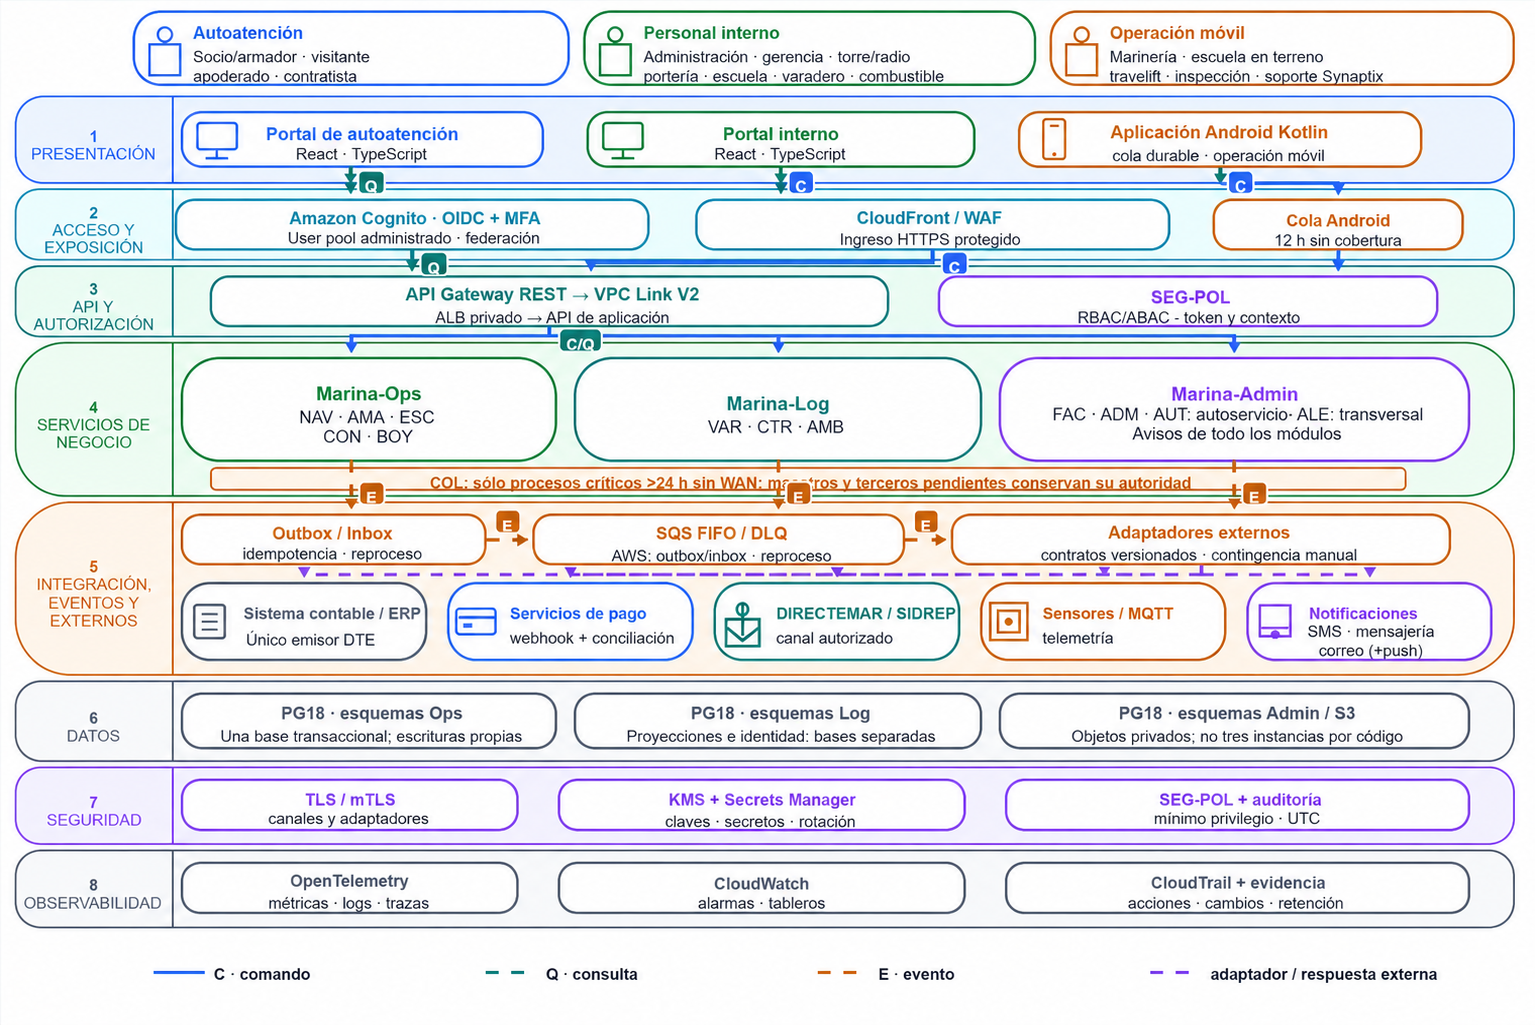
\includegraphics[width=\linewidth,height=.78\textheight,keepaspectratio]{figuras/r8-figura-01.png}
\caption{Descomposición lógica y capas.}
\label{fig:r8-1}
\FuenteFigura{Elaboración propia. Vista de diseño sujeta a verificación de sitio, ingeniería y ensayo.}
\end{figure}
\end{paginaHorizontalSynaptix}\end{quote}
\subsubsection*{Integración, contratos y consistencia}
Las llamadas humanas usan OIDC Authorization Code con PKCE. Los servicios usan OAuth con credenciales de cliente de vida corta o mTLS y un identificador distinto al de personas/dispositivos. Se aplica el perfil de seguridad solicitado para OAuth 2.1, sin atribuir una certificación nominal a productos. Las operaciones REST/JSON se documentan con OpenAPI 3.1; eventos con AsyncAPI 3.0. La especificación se genera y valida en CI y se publica junto al artefacto. Versiones mayores conviven; la deprecación se comunica al menos seis meses antes. Cambios de significado requieren versión aunque el campo conserve nombre.

El catálogo del anexo cubre contable/DTE, autoridad marítima, meteorología/avisos oficiales, portería, cámaras/NVR, medidores, surtidor, boyas, pagos, SMS/mensajería/correo/push, firma, residuos/autoridad sanitaria y canal de baja capacidad. Protocolos existentes de la marina requieren inventario: se oferta MQTT 5 sobre TLS para dispositivos nuevos y HTTPS para negocio; no se afirma que la estación de 2011, portones o NVR tengan una interfaz no acreditada. Un adaptador anticorrupción transforma su modelo sin propagar campos propietarios al núcleo.

El contable existente es el único emisor de DTE. FAC envía hechos aprobados con clave idempotente, conserva recepción/estado de procesamiento y concilia folio/resultado; no atribuye emisión tributaria a la plataforma. La autoridad conserva la autorización oficial de zarpe. Si no existe API autorizada, se prepara/exporta un archivo compatible, se registra intervención/acuse y se mantiene la operación pendiente. DIRECTEMAR/SIDREP, residuos y esquema ambiental deben verificarse con la contraparte antes de publicar formatos definitivos.

Una escritura exige Idempotency-Key UUID, actor autorizado, agregado y versión. Se persiste resultado por 30 días; repetir la misma clave/carga devuelve el mismo resultado y un contenido distinto devuelve 409. La unicidad por agregado se conserva durante su retención, aunque expire la caché del resultado. Outbox guarda hecho y evento en la misma transacción; un trabajador drena lotes de 100, confirma sólo tras entrega y reintenta. Inbox con restricción única protege al consumidor. Hay entrega al menos una vez, orden por agregado, DLQ y reproceso aprobado/auditado. El identificador de correlación viaja desde móvil a COL, nube y terceros.

El perfil interactivo fija conexión $\leq$2 s y respuesta $\leq$5 s; consultas internas críticas tienen deadline $\leq$500 ms, presupuesto distribuido y respuesta de escritura $\leq$800 ms bajo peak. No se añaden reintentos ocultos al camino interactivo: una operación que excede presupuesto queda pendiente y continúa asíncronamente. Trabajadores externos usan timeout 10 s y reintentos a 2, 4, 8, 16 y 32 s con jitter $\pm$20 \%, límite de cinco intentos antes de DLQ. Un circuit breaker abre 30 s tras cinco fallas consecutivas y admite una prueba; cada adaptador tiene pool propio de hasta diez conexiones y cola limitada. Las cuotas concretas de cada tercero se ajustan dentro del catálogo antes de contratar; la campaña de emergencia exige capacidad de aceptación de al menos dos envíos/s por canal.

Las sagas conservan estados: solicitud, validada, reservada, confirmada, compensación o excepción. Una reserva de amarra fallida libera el bloqueo; un pago externo no confirmado no acredita deuda saldada; un fallo de aviso no revierte una transacción válida. Las importaciones masivas validan esquema antes de aplicar, informan errores por fila, admiten procesamiento parcial explícito y exportan asíncronamente CSV/JSON con filtros, autorización, huella y auditoría. El sistema de 2014 se extrae desde copia protegida, con acceso de sólo lectura y acompañamiento de la operadora; se conserva consulta histórica y reversión conforme a SD5, sin ofrecer una integración permanente no requerida.

La figura 4.2 muestra integraciones y límites de confianza. Amazon Cognito es la dependencia administrada de autenticación del gateway y las aplicaciones. SEG-POL aplica autorización contextual. Las bases y el broker local permanecen privados; el contable y la autoridad marítima conservan sus atribuciones externas.

\begin{quote}\small \begin{paginaHorizontalSynaptix}
\begin{figure}[H]
\centering
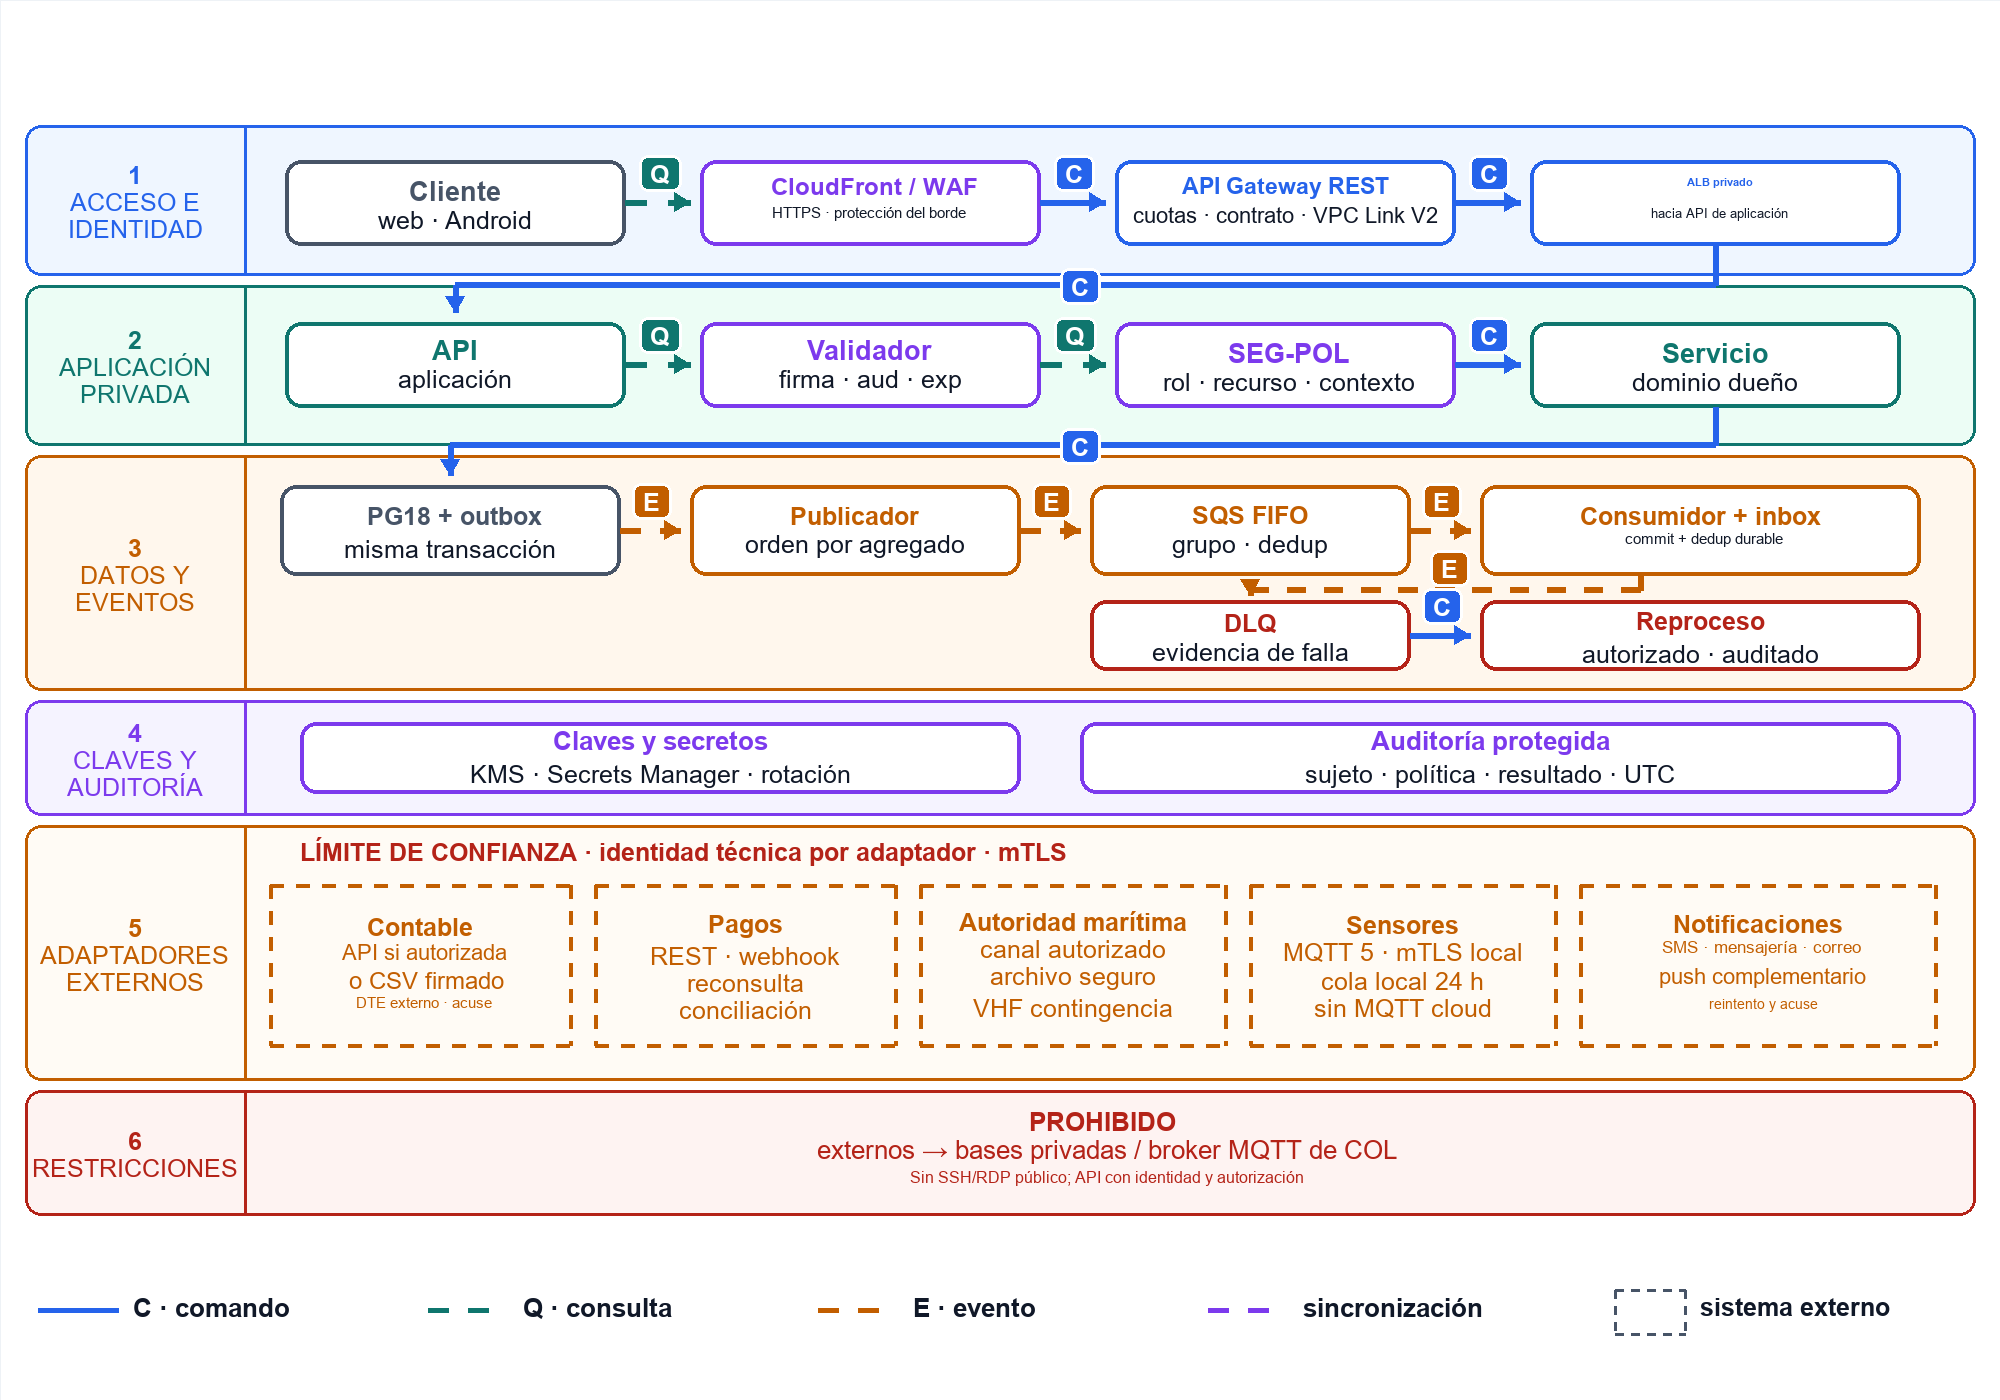
\includegraphics[width=\linewidth,height=.78\textheight,keepaspectratio]{figuras/r8-figura-02.png}
\caption{Integración y seguridad.}
\label{fig:r8-2}
\FuenteFigura{Elaboración propia. Vista de diseño sujeta a verificación de sitio, ingeniería y ensayo.}
\end{figure}
\end{paginaHorizontalSynaptix}\end{quote}
\subsubsection*{Seguridad, privacidad e identidad}
Zero Trust aplica verificación por solicitud, mínimo privilegio y presunción de compromiso. SEG-POL decide según rol, recinto, turno, relación con la nave/alumno, vigencia y sensibilidad; gateway/aplicaciones/objetos actúan como puntos de aplicación. La matriz de controles del anexo relaciona NIST SP 800-207, ISO 27001/27002/27017/27018, NIST CSF 2.0, OWASP ASVS nivel 2, API Security y CIS con implementación y prueba. El análisis STRIDE cubre componentes e integraciones: suplantación, alteración, repudio, divulgación, denegación y elevación de privilegio, actualizado en cada cambio de frontera (Rose et al., 2020).

Se selecciona Amazon Cognito como servicio administrado de identidad, con user pool, OIDC, MFA y federación SAML/OIDC cuando exista un directorio autorizado por el cliente. El identificador de negocio se conserva fuera de Cognito y se vincula al identificador estable del usuario. Los flujos usan Authorization Code con PKCE, validación de emisor, audiencia, estado y nonce; no se admiten flujos implícitos ni tokens en URL. El cierre de sesión revoca la familia de refresh tokens; los tokens de acceso duran cinco minutos, el refresh es rotatorio, la inactividad máxima es de 15 minutos y la jornada máxima de ocho horas. Se limitan a dos sesiones por persona y se prohíben cuentas compartidas. Altas y bajas estacionales se operan como servicio y la baja efectiva debe ocurrir en $\leq$24 horas. La continuidad usa un user pool de contingencia preconfigurado en la región de recuperación: las identidades federadas vuelven a autenticarse y las cuentas no federadas siguen un enrolamiento de recuperación probado; no se afirma réplica de contraseñas entre regiones.

FIDO2 con verificación local del usuario se utiliza en terreno; PIN/biometría más posesión sólo se declara MFA si el ensayo acredita ambos factores. Administradores y accesos externos requieren MFA resistente al phishing; la recuperación usa credenciales enroladas y control reforzado, nunca SMS como única dependencia offline. Los paquetes de autorización están firmados por dispositivo/turno, con duración máxima de 24 h en COL y 12 h en móvil. Se precargan revocaciones; durante aislamiento no se amplían permisos. Operaciones sensibles requieren doble control local; al reconectar se revocan sesiones y se concilian hechos. La elevación privilegiada dura $\leq$60 min, requiere aprobación y grabación. Una cuenta de emergencia de custodia doble se activa por incidente y se revisa dentro de 24 h.

Monitor sólo consulta advertencias de salud indispensables, alumnos de su clase y vigencia de autorización; portería consulta identidad/retiro, no ficha clínica; torre consulta documentación de nave y contacto operacional; varadero/surtidor consultan orden/habilitación, no salud; armador ve sus naves/cuentas; apoderado sólo sus menores; contratista sólo su empresa/faenas; gestor sólo lotes asignados; charter sólo datos contractualmente habilitados; gerencia usa indicadores y excepciones autorizadas; soporte no recibe contenido sensible por defecto. Toda consulta a salud, menores, posición consentida y deuda se audita con propósito, actor, rol, dispositivo, instante UTC/zona, resultado y objeto; cambios incluyen antes/después protegidos.

TLS 1.3 y HSTS con precarga protegen canales web; certificados se renuevan automáticamente con avisos 30/14/7 días antes del vencimiento. Segmentos industriales sin TLS quedan confinados en OT y usan gateway cifrado, ACL y monitoreo compensatorio. AES-256 protege volúmenes, móviles, objetos y respaldos. Además, salud, datos personales de menores, armadores/tripulantes/contratistas y posición voluntaria se cifran por campo con AES-256-GCM, claves de datos por categoría y envoltura KMS; la búsqueda usa identificadores no sensibles o índices protegidos, nunca copias claras generales. Claves se rotan anualmente y tras incidente; custodia, operación y auditoría están segregadas. Respaldos tienen claves/cuenta independientes y recuperación de claves ensayada.

CDN/WAF/DDoS combinan protección L3/L4 del proveedor, reglas L7 administradas/propias, límites de cuerpo, bot/rate limiting y origen restringido; las rutas privadas o alternativas no evitan esas políticas. El SOC gestionado 24$\times$7 recibe SIEM y telemetría de endpoints/cargas; eventos locales se almacenan durante corte y se remiten luego, sin prometer detección remota instantánea. Logs de seguridad se mantienen 12 meses en línea y 24 adicionales archivados. Auditoría de negocio tiene al menos cinco años o mayor plazo aplicable; no se registran tokens, salud ni contraseñas en logs técnicos.

Se comunica incidente crítico dentro de dos horas, brecha dentro de 24 h e informe preliminar/causa raíz en cinco días hábiles. Se aíslan dispositivo/carga y se recupera desde imagen/copia íntegra. Vulnerabilidades: máximos de siete días corridos críticas, 15 altas y 30 medias desde publicación/detección; explotadas requieren mitigación en 24 h. El congelamiento estacional admite intervención urgente aprobada y reversible. Pentest independiente antes de cada paso a producción y anual; ningún hallazgo crítico/alto abierto permite promoción.

Datos principales/objetos/identidad/respaldos se ubican en Chile y Brasil según el proveedor activo. CDN, planos de control, SOC, firma, mensajería y lectura documental pueden introducir tratamiento adicional: cada proveedor se registra como subencargado con ubicación, finalidad y autorización previa escrita. No se declara autorización ya obtenida. Consentimientos voluntarios son granulares, versionados y revocables; revocación detiene nueva captura/consulta/envío de posición, preservando conservación obligatoria. El registro de tratamientos, evaluación de impacto cuando proceda, derechos y eliminación se revisan con el cliente; no se habilita transferencia sensible por el solo hecho de seleccionar un servicio.

\subsubsection*{Datos, capacidades transversales y operación desconectada}
PostgreSQL 18 almacena hechos transaccionales y maestros; una instancia separada mantiene proyecciones de lectura reconstruibles y la analítica consulta archivos abiertos Parquet/objetos sin cargar el primario. COL conserva PostgreSQL del subconjunto autorizado y móviles SQLite cifrado. La caché de aplicación es reconstruible, expira a 60 s y no decide asignaciones, salud, consentimiento ni permisos; deuda/asistencia se consultan contra su autoridad. Índices por UUID/tiempo/estado, particiones mensuales para lecturas y eventos y controles ISO 25012 se concilian con SD5.

El dato operacional de COL conserva autoridad sobre hechos de recinto; maestros contractuales cloud mantienen versión. No se aplica última escritura gana a retiros, combustible, asignación, deuda o custodia. Retiro autorizado prevalece sobre asistencia antigua; despacho ya confirmado se preserva y duplicados se descartan; conflictos comerciales quedan en bandeja con responsable y SLA. Se conservan event\_id, versión, secuencia por agregado, actor/dispositivo, UTC y offset de reloj; un reloj desviado >60 s se marca y exige conciliación. Commit local durable antecede a confirmación; reinicio recupera WAL/cola sin perder hechos reconocidos.

Paquetes locales incluyen naves/contratos vigentes, documentación de zarpe, recursos/compatibilidad, escuela del turno, autorizaciones, existencias/órdenes, contactos de emergencia y políticas. COL sigue 24 h recepción/asignación, salida/regreso, preparación de zarpe, combustible y escuela. Móvil permite 12 h de captura de turno y boyas ocho horas. Nuevos permisos maestros, pagos externos, DTE, autorización oficial y entrega remota no se confirman sin contraparte; se ofrece solicitud pendiente, comprobante provisional y revisión al reconectar. Ningún terminal aislado confirma una asignación exclusiva sin COL/torre ni autoriza a un menor con información remota potencialmente desactualizada.

El retiro anticipado se registra y difunde inmediatamente en LAN. Si el monitor está fuera de cobertura, el protocolo exige confirmación por radio con portería antes de una nueva salida y conciliación de nómina; sin confirmación se bloquea esa salida. «Escuela en tiempo real» se mide para información confirmada del recinto; una interfaz remota aislada indica indisponibilidad y exige canal compensatorio, no se presenta como tiempo real.

La sincronización de aplicación móvil--COL y COL--nube usa REST/JSON sobre HTTPS/mTLS, lotes de hasta 100 hechos con checksum, secuencia y acuse posterior a commit. Emisor conserva lote hasta acuse; duplicados devuelven resultado anterior. Se vacía backlog crítico antes de objetos/video/analítica, con 1 Mbit/s útil reservado. El límite contractual es $\leq$30 min después de 24 h de corte, medido hasta aplicación/conciliación automática de registros válidos, no sólo hasta transmisión.

La actualización de ocupación es $\leq$60 s desde evento observado/confirmado; consumos se actualizan al menos cada hora; cuenta y situación escolar en tiempo real cuando su autoridad está alcanzable; ambiente consolida diariamente. Los límites durante cortes se muestran por origen/antigüedad. Retención: menores hasta 18 años +5 y mínimo diez años; movimientos/zarpe cinco; contratos/custodia/cuentas seis; residuos/derrames seis; consumo cinco; combustible cinco; tren de fondeo vida útil +5; CCTV seis meses, al menos 30 días en línea donde aplica. Consentimientos sobreviven cinco años tras último uso salvo mayor necesidad probatoria; avisos, acreditaciones, contactos y planes siguen plazo del expediente relacionado; telemetría cruda cinco años y agregados diez como oferta de diseño. Evidencia contractual se conserva contrato +24 meses. Legal hold suspende borrado (PUCV, 2026c, cap. 15, RT-05.10; PUCV, 2026a, art. 27).

La exportación completa CSV/JSON/Parquet más objetos/manifiestos es autoservida, asíncrona y sin cargo adicional por extracción; se auditan exportaciones sensibles. Borrado genera tombstone durable que viaja a COL/móviles/réplicas; respaldos expiran según ciclo aprobado y una restauración reaplica tombstones antes de abrir acceso. Se conservan certificados de sanitización y excepciones por conservación legítima.

Administración funcional configura usuarios/unidades, catálogos, reglas y umbrales con versión; cambios críticos requieren doble aprobación. Una bandeja unificada conserva responsable, plazo, delegación y escalamiento. Búsqueda global usa índice separado con filtros de acceso evaluados al consultar; paginación y exportación conservan filtros. El portal público se sirve desde recursos separados de transacciones; ofrece disponibilidad no exclusiva, condiciones y tarifas administradas del cliente sin inventar montos. Autoservicio de armador/apoderado/contratista registra solicitud/pago/estado. Como hipótesis inicial, si 300 de 1.000 consultas mensuales son aptas y 60 \% se resuelven sin mesa, reducción estimada =180/1.000=18 \%; se valida con conteos reales y no se presenta como ahorro observado.

Firma/documentos conservan metadatos, versiones, permisos, preview, plantillas, huellas, certificado y sello de tiempo verificable tras vencimiento. Se propone un prestador chileno acreditado para firma avanzada cuando el acto lo requiera; el proveedor concreto y modalidad por contrato/autorización/custodia/izaje/residuo quedan como selección externa pendiente, no como contratación acreditada. Avisos obligatorios no admiten baja comercial; campañas comerciales sí, con preferencias versionadas. Se distinguen aceptado, entregado, leído cuando el canal lo permita y sin acuse.

La figura 4.3 muestra autoridad de datos y sincronización. COL opera 24 horas sin nube, con permisos sujetos a vigencia y revocación; los terminales móviles mantienen 12 horas y la inspección de boyas ocho horas. La conciliación en 30 minutos es un objetivo por ensayar.

\begin{quote}\small \begin{paginaHorizontalSynaptix}
\begin{figure}[H]
\centering
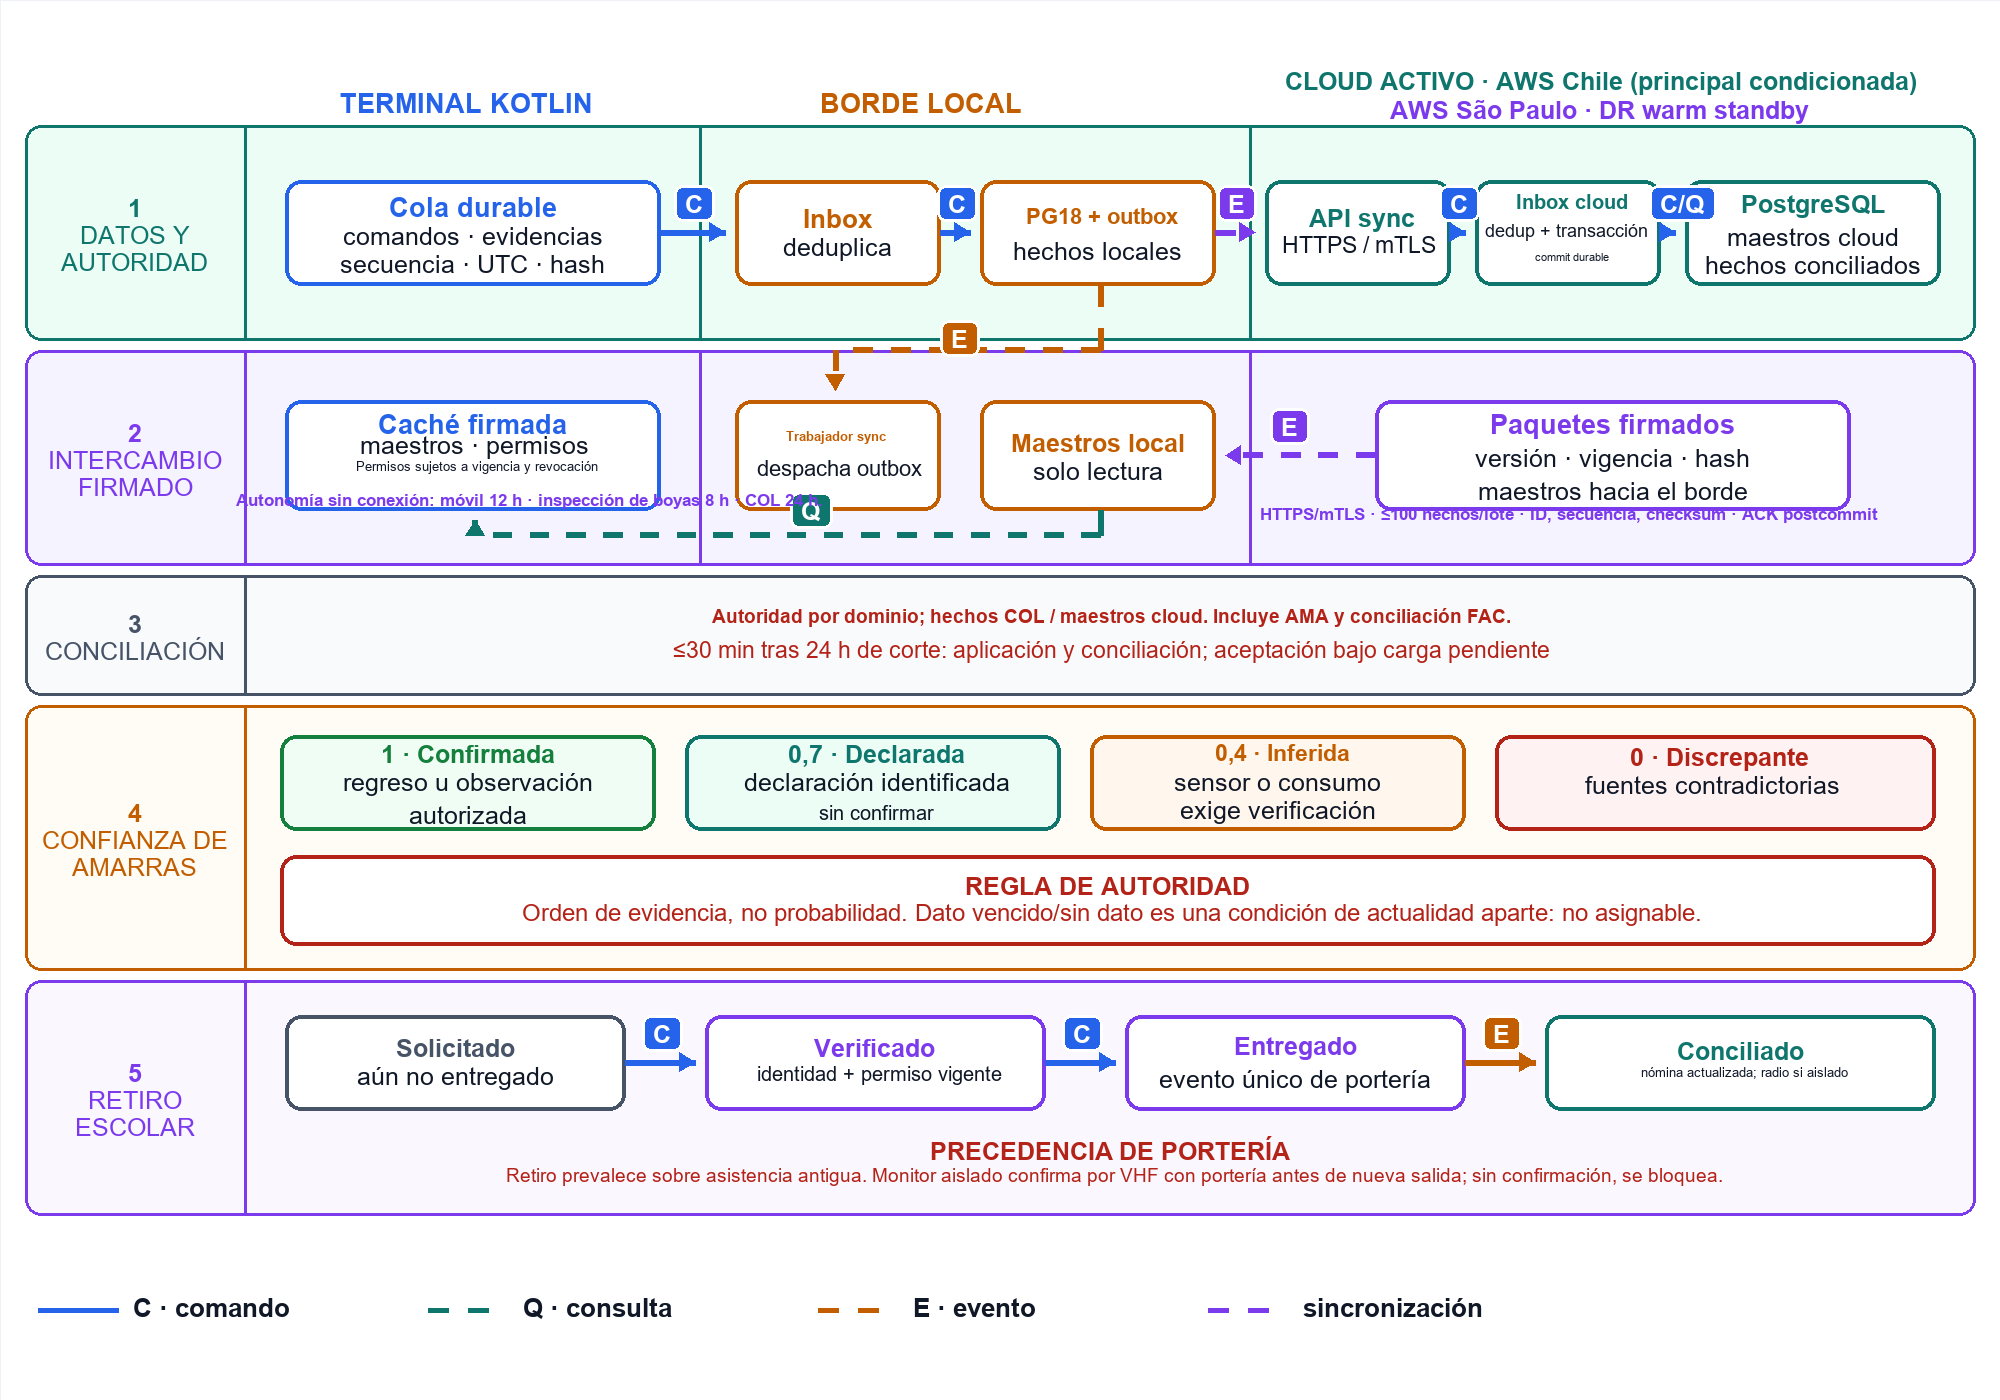
\includegraphics[width=\linewidth,height=.78\textheight,keepaspectratio]{figuras/r8-figura-03.png}
\caption{Autoridad, confianza y sincronización.}
\label{fig:r8-3}
\FuenteFigura{Elaboración propia. Vista de diseño sujeta a verificación de sitio, ingeniería y ensayo.}
\end{figure}
\end{paginaHorizontalSynaptix}\end{quote}
\subsubsection*{Procesos críticos y aceptación}
\begin{table}[H]
\centering
\small
\appto\EstiloTablaSynaptix{\fontsize{8}{9.5}\selectfont\renewcommand{\arraystretch}{1.15}\setlength{\extrarowheight}{0pt}}
\begin{tabularx}{\linewidth}{|p{.19\linewidth}|p{.35\linewidth}|X|}
\hline
\EncabezadoTabla{Proceso} & \EncabezadoTabla{Regla y falla controlada} & \EncabezadoTabla{Criterio de diseño/prueba} \\ \hline
Amarra/salida/regreso & Declaración, observación autorizada y señales de presencia; presencia no identifica nave. Torre confirma identidad y discrepancias. & Registro $\leq$10 s/dos interacciones; ocupación $\leq$60 s desde hecho confirmado. \\ \hline
Plan vencido & Armador informa ETA; vencimiento =ETA registrada, sin gracia oculta; cierre exige evidencia humana válida. & Alerta $\leq$15 min desde vencimiento; torre escala y conserva «sin noticias». No se sustituye SAR ni permiso de zarpe. \\ \hline
Marejada & Aviso oficial verificado suspende actividades; 296 armadores reciben SMS, mensajería y correo simultáneos. & 888 envíos iniciales; último envío $\leq$600 s; reintentos y llamada registrada sin acuse. \\ \hline
Escuela & Nómina alumno--bote--monitor, autorización vigente, cambio de bote/monitor y recuento de regreso. & Hasta 18 botes $\leq$60 s; excepción por persona ausente y aviso al apoderado. Sin cámaras/dispositivos en menores ni botes menores. \\ \hline
Visitante por VHF & Torre compara eslora/manga/calado a marea baja, exposición y reserva única; registra estadía nocturna/hecho facturable. & Asignación y confirmación $\leq$45 s; excepción auditada; lista de espera por antigüedad y compatibilidad con aprobación comercial. \\ \hline
90 zarpes sin WAN & Legajos/permisos previos, validación humana, ID único, impresión/exportación y cola. & Nómina/legajo $\leq$90 s; se mide atención humana aparte; cero pérdida/duplicados al volver. \\ \hline
Izaje/invernada & Ficha/plan aprobados antes de maniobra; registro posterior seguro en calzos; posición y orden de botadura. & Sin interacción con carga suspendida; clima bloquea/reprograma y avisa. \\ \hline
Contratista/residuo & Portería valida empresa/persona, vigencia y capacitación; personal del puerto captura lote/faena/nave. & 62 empresas/140 personas iniciales; ninguna app obligatoria al contratista; evidencia de entrega al gestor. \\ \hline
Surtidor & Captura manual controlada en puesto seguro mientras se acredita instrumentación de zona; operador/volumen/nave/existencia. & Conciliación diaria con contador/existencia, doble revisión de ajuste; continuidad COL y suspensión por clima. \\ \hline
Consumo & Dos puntos de servicio por amarra; lectura ausente/anómala, calibración/cambio/ajuste autorizado. & Fuente única cobro/ambiente, atribución verificable; serie ambiental temprana para 2029. \\ \hline
Boyas & Paquete por tren de fondeo, inspección y evidencia; ocupación/identidad por declaración y confirmación al asignar. & Ocho horas offline; una ronda antigua no prueba actualidad. Recursos sin confirmación quedan indeterminados/no asignables. \\ \hline
Mora/abandono & Expediente íntegro de 14 naves, deuda/custodia y revisión comercial. & Ningún bloqueo por deuda automático sin decisión formal fundada; sin cobranza judicial incluida. \\ \hline
\end{tabularx}
\caption{Procesos críticos y aceptación}
\label{tab:procesos-criticos}
\FuenteTabla{elaboración propia conforme a PUCV (2026c, §§16.1, 17.4 y cap. 18)}
\end{table}
Los procesos de seguridad tienen contingencia conservadora; las aplicaciones no inventan permisos por ausencia de enlace.

El modelo de confianza distingue confirmado, declarado, inferido y discrepante; los valores 1/0,7/0,4/0 son etiquetas de orden y no precisión medida. Para responder a DEC-01 se plantea un piloto opcional de 20 posiciones ---cuatro por pantalán--- durante 30 días, con observación de referencia en 200 transiciones equilibradas y distintos estados de marea/oleaje. La meta de diseño es $\geq$95 \% de concordancia de presencia, falsos libres $\leq$1 \% y ninguna asignación exclusiva basada sólo en la señal. La selección del sensor y su aptitud marina se aceptan mediante ficha y ensayo. La función obligatoria de ocupación permanece sustentada por la bitácora operacional y la ronda física registrada; el piloto no condiciona su operación ni autoriza por sí solo un despliegue masivo.

El canal de baja capacidad se propone compatible con mensajes Iridium/SBD de equipo ya disponible del armador, mediante pasarela del proveedor que éste utilice; no se incluye compra obligatoria a bordo. Antes de contratar se verifica compatibilidad/autorización. Sobre de diseño $\leq$250 bytes con ID, secuencia, tiempo, vigencia, tipo y autenticador; el límite es propio del diseño y no se atribuye a todo servicio satelital. La fecha del evento gobierna vigencia; mensaje tardío no cierra regreso ni cancela alerta. Los timeouts del transporte se fijarán con su contrato de latencia de horas. El escalamiento operacional por ETA/alerta no espera al transporte. Ausencia de acuse mantiene «no entregado/sin noticias» y permite VHF/llamada; no prueba accidente.

Contactos se verifican al renovar y por campaña pretemporada; rebotes/errores originan tarea al responsable comercial. Las 14 naves sin propietario contactable se incluyen en expediente y campaña de búsqueda, sin marcar entrega ficticia. Si un proveedor de avisos cae, se drena por canal disponible y llamada; si cae el contable, hechos esperan y no se duplican; identidad caída conserva permisos locales vigentes; medidor fallado se marca y no se inventa lectura; almacenamiento al 70/80/90 \% dispara ampliación/alarma/degradación, conservando siempre hechos críticos.

\subsubsection*{Interfaces, movilidad y observabilidad}
Las interfaces se diseñan para WCAG 2.2 AA, con EN 301 549 complementaria, teclado completo, foco visible, alto contraste, icono más texto y objetivos táctiles $\geq$44$\times$44 px. Funciones principales quedan a $\leq$3 interacciones; registro de pantalán a dos y $\leq$10 s. Meta inicial: error de registro $\leq$2 \% y aprendizaje del flujo básico $\leq$30 min por perfil, a validar antes de construcción final. Pantalla mojada, guantes, sol y semirrígido se ensayan con dispositivo real; no se exige interacción durante amarre/izaje. El sistema de diseño usa la paleta Synaptix, una familia sans y componentes compartidos. Inglés y español cubren canales de visitantes, tripulantes extranjeros y charter y mesa de temporada; no se impone inglés a todas las pantallas internas.

Pendiente, confirmado local, aceptado por tercero, desactualizado, error y degradación tienen mensajes distintos. Pruebas automatizadas de accesibilidad se combinan con teclado/lector de pantalla y usuarios reales por perfil; resultados no se inventan. NOC 24$\times$7$\times$365 controla plataforma y planes vencidos/emergencia; mesa 06:00--24:00 en temporada y 08:00--20:00 el resto, con críticos/altos 24$\times$7. El SOC se coordina por ITSM. Synaptix aporta guardia de operación y especialistas; la marina sólo valida decisiones funcionales.

OpenTelemetry SDK/agentes $\rightarrow$ colector local/cloud $\rightarrow$ almacén del proveedor activo conserva trace\_id común. Métricas incluyen transacción completa, p95, backlog, retraso de réplica, batería/disco/enlace y síntomas de negocio. El cliente recibe cuenta propia permanente y exportación. Logs técnicos 30 días en línea/180 archivados, métricas 13 meses y trazas 30 días, como política inicial dimensionable; seguridad/auditoría siguen sus plazos mayores. COL bufferiza siete días de telemetría operativa además de la cola crítica, sin mezclar retenciones.

Alerta roja: réplica >10 min o aviso de marejada con envío pendiente a los cinco minutos; crítica al incumplir objetivo. Amarilla: lectura ausente dos intervalos, contacto rebotado, cola >15 min, disco >70 \%; roja al 80 \% y contención al 90 \%. Plan vencido y retiro no propagado escalan de inmediato conforme al flujo. Se agrupan por incidente, con acuse en 15 min para crítico y guardia alternativa; supresión sólo por mantenimiento aprobado, nunca de alerta de personas. Los runbooks precisan quién ejecuta aislamiento, restauración, cambio WAN, ampliación y comunicación.

Presupuesto mensual crítico 99,9 \%: con 30 días, 43,2 min de indisponibilidad. Al consumir 50 \% se limita despliegue; a 100 \% se permiten sólo recuperación/seguridad. Reporte mensual y causa raíz en cinco días hábiles; capacidad se proyecta trimestralmente. Indicadores de entrega: cambios fallidos $\leq$5 \% mensual, restauración crítica $\leq$4 h, objetivo semanal de liberación fuera de freeze y lead time $\leq$cinco días hábiles, medidos en CI/ITSM.

\subsection{Especificaciones Tecnologías de Software a utilizar}
La oferta mantiene una línea de construcción común entre proveedores; cambia el adaptador de plataforma sólo cuando se aprueba la alternativa. No se mantiene un inventario productivo simultáneo de AWS y GCP. La lista técnica distingue versiones verificadas, condiciones de servicio gestionado y actualizaciones necesarias hasta mes 56.

\begin{table}[H]
\centering
\small
\begin{tabularx}{\linewidth}{|p{.28\linewidth}|X|}
\hline
\EncabezadoTabla{Responsabilidad} & \EncabezadoTabla{Selección de diseño y soporte} \\ \hline
Backend & Java 21 LTS, Spring Boot 4.1 y Spring Modulith 2; BOM de minor/parches compatible y digest antes de H2. Soporte comercial o mantenimiento Synaptix y actualización anual; no se inventa EOS de toda la cadena. \\ \hline
Datos & PostgreSQL 18, misma major cloud/COL; fin comunitario 14-11-2030. Actualización mayor ensayada al menos seis meses antes de EOS y antes si horizonte contractual lo exige. \\ \hline
Presentación & React/TypeScript web; Kotlin Android nativo y SQLite cifrado para terreno. Licencias OSS inventariadas por dependencia; minor fijadas en lockfile/BOM. \\ \hline
Identidad & Amazon Cognito con user pool, OIDC, MFA y federación; configuración versionada, exportación de atributos permitidos, revisión semestral y prueba del pool de contingencia. \\ \hline
AWS aprobado & ECS/Fargate, RDS PostgreSQL, S3, SQS FIFO/DLQ, API Gateway REST/VPC Link V2, ALB privado, CloudFront/WAF/Shield, KMS, Secrets Manager, CloudWatch/CloudTrail. Cada servicio debe pasar G-REG. \\ \hline
GCP aprobado & Cloud Run, Cloud SQL PostgreSQL, Cloud Storage, balanceador/Cloud Armor/CDN, gateway HTTPS en aplicación, outbox/inbox PostgreSQL, Compute Engine para identidad, KMS/Secret Manager y Logging/Monitoring. Gate de equivalencia antes de activar. \\ \hline
COL & Ubuntu Server 24.04 LTS, Podman/systemd, Pacemaker/Corosync y testigo independiente; réplica PostgreSQL síncrona, fencing por energía/gestión. BOM compatible antes de compra. \\ \hline
Construcción & Git protegido, JUnit/Testcontainers, Flyway, OpenAPI/AsyncAPI, SBOM CycloneDX, firma de imágenes y Terraform versionado con estado cifrado/bloqueado. \\ \hline
Operación & OpenTelemetry, SIEM/EDR y MDM gestionados como servicio; prestadores/SKU/retenciones de contrato pendientes de acreditar, sin declarar licencia adquirida. \\ \hline
\end{tabularx}
\caption{Tecnologías y soporte}
\label{tab:tecnologias-soporte}
\FuenteTabla{diseño propio y documentación técnica oficial consultada el 10 de octubre de 2026}
\end{table}
Las versiones citadas no acreditan automáticamente soporte de región, distribución, dispositivo o plugin: la BOM y G-REG verifican esa combinación.

Servicios gestionados sin EOS público se controlan por soporte contractual, ciclo de API y aviso de deprecación, con sustitución ensayada antes del cambio. Java/Ubuntu requieren soporte vigente que cubra mes 56; la fecha absoluta de término depende de M1 aprobado. React/TypeScript/Kotlin/herramientas siguen actualización trimestral y revisión de seguridad continua. El anexo conserva proveedor, licencia, evidencia, próxima revisión y ruta de sustitución; las garantías de terceros todavía no celebradas quedan pendientes reales.

Android cubre versión vigente y dos anteriores según RT-17.03, con matriz por SKU/patch y fecha de soporte del fabricante; no se deduce EOS de Android. Flota usa distribución corporativa firmada, MDM, cifrado, bloqueo/borrado al reconectar, inventario, batería por turno y objetivo de transmisión $\leq$250 MB/turno salvo evidencia multimedia autorizada. Portal prueba Chrome/Edge/Firefox/Safari vigentes y dos anteriores cuando soportados. La app de terreno es nativa; portal web no sustituye la cola/credencial local.

CI exige revisión por pares y prohíbe escritura directa al principal; une requisito--incidencia--commit--prueba--despliegue. Pipeline ejecuta compilación, pruebas de contrato/negocio, SAST/SCA/secretos/contenedores/DAST, cobertura $\geq$70 \% de lógica de negocio, SBOM y procedencia SLSA $\geq$3 con runner aislado y firma protegida. Hallazgos críticos/altos, contrato roto o licencia no aprobada bloquean. OWASP SAMM gobierna madurez y revisión de dependencia por mantenimiento/soporte/licencia. El repositorio pertenece al cliente, se actualiza por liberación y se deposita en custodia independiente semestral.

Un mismo artefacto se promueve sin recompilar, con configuración externalizada y secretos por ambiente. Se selecciona despliegue progresivo 10/50/100 \% con pausas y verificación de error/p95; rollback automático a digest previo. Esquemas usan expand--contract, convivencia de dos versiones y backfill; migración irreversible requiere avance seguro/restore, no una reversión ficticia. IaC se revisa por pares, conserva estado remoto cifrado/bloqueado, detecta drift diariamente y reproduce ambientes. PREPROD prueba upgrade/rollback antes de PROD.

Las innovaciones IN1/IN2/IN4/IN5 usan reglas/flujo/analítica determinista según su alcance. IN3 propone extracción documental asistida; campos extraídos son sugerencias hasta aprobación humana, sin autorización automática de nave/persona. Modelo/prestador/versión y residencia se deben individualizar antes de procesar datos reales; documentos sensibles no se envían fuera de ubicaciones autorizadas. Se bloquea entrenamiento de terceros sin autorización, se registran versiones/errores, se evalúa sesgo por tipo documental, se mide precisión por campo contra referencia humana y se desactiva a captura manual sin afectar el servicio. Se gobierna con NIST AI RMF/ISO 42001; no se presenta una métrica o certificación como obtenida.

\section{Arquitectura física}
El despliegue asigna cada componente lógico a ubicación, recurso, ambiente y etapa. La preferencia por servicios administrados reduce carga técnica; COL e identidad portable requieren administración especializada de Synaptix por necesidad de continuidad y reversibilidad. El Anexo A4 identifica unidades, almacenes, elementos transversales, innovaciones y recursos; la implementación de cada componente se acredita mediante las pruebas y evidencias de aceptación correspondientes.

\subsubsection*{Ambientes y despliegue regional}
Desarrollo, QA, Preproducción, Producción y DR se habilitan en H3/mes 6 dentro del proveedor aprobado, en cuentas/proyectos, redes, datos y credenciales aislados. H2/mes 4 cierra arquitectura/seguridad/datos; G-REG debe decidirse antes de H3. PREPROD reproduce versiones, topología de dos zonas y mecanismos de DR; usa carga sintética representativa, no datos reales de menores. DEV/QA tienen menor capacidad justificada y se apagan fuera de uso; las diferencias no se extrapolan como prueba de HA productiva.

En AWS la región Chile, su código y dos AZ físicas se acreditan en G-REG; São Paulo usa sa-east-1. No se sustituye una región por una Local Zone. Producción usa VPC 10.20.0.0/16, DEV 10.21.0.0/16, QA 10.22.0.0/16, PREPROD 10.23.0.0/16 y DR 10.24.0.0/16; se verifica no solapamiento. Subredes de aplicación/datos privadas en dos AZ, NAT por AZ, endpoints privados y ALB interno; ingreso público CloudFront/WAF $\rightarrow$ API Gateway REST regional $\rightarrow$ VPC Link V2/ALB $\rightarrow$ servicios. Amazon Cognito emite tokens OIDC que el gateway y las aplicaciones validan; RDS no tiene IP pública.

En la alternativa GCP el primario es southamerica-west1 y DR southamerica-east1. VPC/proyectos y rangos no se solapan; Cloud Run administra distribución zonal, Cloud SQL se configura HA y Compute Engine de identidad usa dos zonas. No se atribuye selección de zona al operador de Cloud Run. Balanceador/Cloud Armor protegen el ingreso, gateway aplica contratos/cuotas antes de módulos y los endpoints directos se restringen. La equivalencia se verifica por prueba; no se confunde un API Gateway gestionado de un proveedor con el otro ni se transporta SQS directamente a Pub/Sub.

La figura 4.4 presenta la arquitectura física general: COL A/B, red segmentada, fibra GTD/Telsur y respaldo Starlink, Amazon Cognito y mensajería SQS. El almacenamiento auxiliar sirve a copias y staging y no aloja datos transaccionales. AWS Chile está condicionado a G-REG; la alternativa GCP exige aprobación y no opera simultáneamente.

\begin{quote}\small \begin{paginaHorizontalSynaptix}
\begin{figure}[H]
\centering
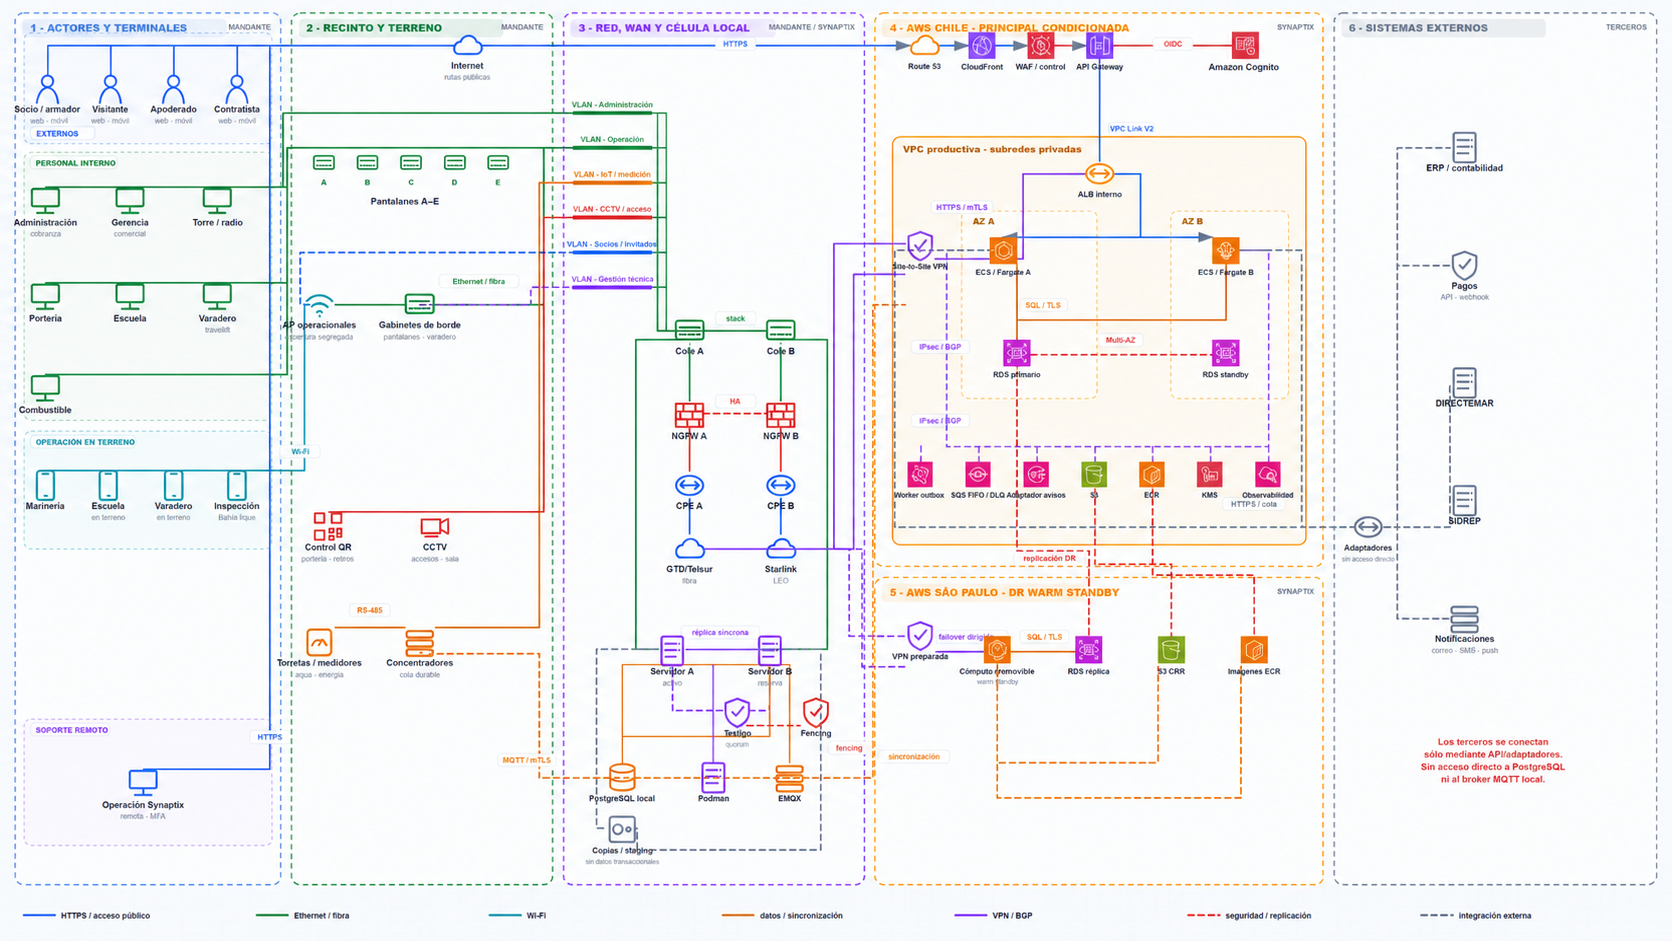
\includegraphics[width=\linewidth,height=.78\textheight,keepaspectratio]{figuras/r8-figura-04.png}
\caption{Arquitectura física general.}
\label{fig:r8-4}
\FuenteFigura{Elaboración propia. Vista de diseño sujeta a verificación de sitio, ingeniería y ensayo.}
\end{figure}
\end{paginaHorizontalSynaptix}\end{quote}
Etapa 1 se construye meses 1--12, marcha blanca 13--15 y producción desde 16; Etapa 2 desarrollo 13--18, marcha 19--20 y producción desde 21, operación hasta 56. En 13--15 conviven marcha de E1 y desarrollo de E2; en 19--20 producción E1 y marcha E2. Maestros/fuente compartidos evitan doble digitación. Marcha exige cuatro semanas con carga/SLA sostenidos, cero críticos/altos abiertos, conciliación sin diferencias inexplicadas y capacitación/aceptación. Se respetan freeze 15 diciembre--15 marzo, campañas de varadero abril--mayo/septiembre--noviembre, 14 eventos y suspensión de marejada. La instalación de consumos se adelanta para serie 2029 sin posponer hitos; cada actividad se enlaza a un paquete de SD7, que debe actualizarse por el equipo responsable.

\subsubsection*{Capacidad, crecimiento y sensibilidad}
La línea base/proyección del caso se conserva en el siguiente resumen; un punto de servicio no acredita un medidor instalado. Hoy hay cero puntos instrumentados; se oferta medición individual por amarra con dos canales ---agua/electricidad---: 640 iniciales y 760 al ampliar. El número de torretas no se usa como equivalencia automática de puestos (PUCV, 2026c, §14.1, pp. 30--31).

\begin{table}[H]
\centering
\small
\begin{tabularx}{\linewidth}{|p{.28\linewidth}|X|}
\hline
\EncabezadoTabla{Magnitud} & \EncabezadoTabla{Inicial $\rightarrow$ proyección} \\ \hline
Amarras/contratos & 320/296 $\rightarrow$380/350; 28 puestos de visitas incluidos en mapa a conciliar, sin sumarlos dos veces. \\ \hline
Invernada/boyas & 180 puestos, 152 ocupados $\rightarrow$200; 40 boyas $\rightarrow$70. \\ \hline
Recaladas/zarpes/movimientos & 1.900/4.800/1.150 $\rightarrow$2.400/5.600/1.350; peak 90$\rightarrow$110 zarpes. \\ \hline
Combustible/socios & 1,9$\rightarrow$2,2 millones de litros; 1.240$\rightarrow$1.450 socios. \\ \hline
Escuela/eventos & 640 alumnos/470 menores/1.100 clases/14 eventos $\rightarrow$800/590/1.400/18. \\ \hline
Contratistas/torretas/cámaras & 62 empresas/140 personas/168 torretas/38 cámaras $\rightarrow$75/170/200/60. \\ \hline
Cobros/personal/ingresos & 1.950$\rightarrow$2.300 cobros/mes; 39--78$\rightarrow$44--88 trabajadores; 3.400$\rightarrow$4.000 personas distintas/mes. \\ \hline
\end{tabularx}
\caption{Volumetría inicial y proyección}
\label{tab:volumetria-proyeccion}
\FuenteTabla{PUCV (2026c, §14.1)}
\end{table}
El plano debe conciliar tomas, amarras, torretas y muelle antes de instalar; esa conciliación física sigue como antecedente de sitio.

Hipótesis reproducible de peak: 90 zarpes$\times$6 +20 recaladas$\times$8 +250 movimientos$\times$2 +3 clases$\times$22 +40 despachos$\times$3 +12 izajes$\times$5 +400 accesos =1.846 operaciones. Si 40 \% ocurre en una hora, 0,205 operaciones/s; con nueve lecturas por escritura y telemetría de 760 canales cada 900 s, total 2,895 operaciones de datos/s. Base de diseño: tres sostenidas/diez en ráfaga; no son solicitudes HTTP. La exigencia adicional de 3$\times$ inicial en tres años se prueba con nueve sostenidas/30 en ráfaga, 960 amarras/1.920 puntos como envolvente de software, sin obligar compra inmediata de esos equipos. Es distinta de la ampliación comercial 380/70.

Concurrencia de diseño: 35 internos ---12 marina/torre, cinco escuela, cuatro varadero, cuatro administración, dos combustible, cuatro portería y cuatro soporte/gestión--- y 120 externos ---50 armadores, 50 apoderados, diez visitantes, cinco contratistas y cinco charter---. Son hipótesis de simultaneidad, no dotación del caso; se contrastan con turnos y pruebas. El dato 35/120 no se reutiliza como requisito impuesto.

Telemetría: 760$\times$96=72.960 lecturas/día; 26.630.400/año. Con registro 128 bytes y factor tres de índices/metadatos: 10,23 GB/año; cinco años =51,13 GB, al 70 \% máximo =73,05 GB. A 3$\times$ inicial: 1.920$\times$96$\times$365$\times$128$\times$3$\times$5/10\textasciicircum{}9/0,7$\approx$184,54 GB sólo de telemetría. Base transaccional inicial 200 GB, expansión hasta 1 TB; proyecciones físicas separadas 100 GB iniciales, no «15 GB» como instancia que el servicio no oferta. Índices/WAL/otras entidades usan reserva propia y deben medir IOPS/conexiones, no deducirlas de tamaño.

Documentos: hipótesis inicial 60 GB históricos +10.000 documentos/año$\times$2 MB =20 GB/año; seis años nuevos =120 GB, total 180 GB y 257,15 GB con 30 \% reserva. Objetos iniciales 500 GB excluyen video. La migración conserva padrón completo, contratos vigentes, seis años de pagos/saldos, 14 expedientes completos, naves/invernada y tres años de matrícula; el volumen histórico se mide desde copia, no se limita arbitrariamente a 60 GB.

Auditoría: hipótesis 20.000 hechos/día$\times$1 KiB$\times$365$\times$5$\times$2 por índices $\approx$74,75 GB a cinco años. Logs de seguridad: 1 GB/día de diseño $\rightarrow$365 GB en línea +730 GB de archivo, con 1,6 TB de reserva inicial. Métricas/trazas se presupuestan a 250 MB/día cada una según muestreo; volumen se mide y ajusta por política de retención. Estas cotas no se duplican como telemetría transaccional.

CCTV es independiente: 38 cámaras$\times$2 Mbit/s$\times$86.400/8 =820,8 GB/día; seis meses de 180 días $\approx$147,74 TB sin compresión adicional; 30 días en línea $\approx$24,62 TB. Con 30 \% reserva, capacidad útil $\approx$211,06 TB; expansión a 60 cámaras $\approx$333,26 TB. La tasa real, resolución, horarios y codec del NVR deben verificarse; no se oferta este espacio como un SSD del COL ni se transmite video por el respaldo durante vaciado crítico. Una política de tasa diferente debe demostrar evidencia suficiente y retención, no reducirla sólo para abaratar.

Backlog: 72.960 lecturas +1.846 hechos/día =74.806 sobres. Con 1 KiB, 76,60 MB; 30 días$\times$factor tres $\approx$6,89 GB por nodo, reserva de diseño 20 GB. A 1 Mbit/s útil y factor dos de protocolo/reintento: transmisión $\approx$1.226 s; aplicación a 150 hechos/s $\approx$499 s, más 60 s de validación y unas 300 entradas nuevas procesadas en paralelo. Envolvente conservadora $\approx$1.785 s, inferior a 1.800 s por sólo 15 s: se reconoce margen estrecho y se reserva 2 Mbit/s útiles como objetivo operativo, manteniendo prueba límite a 1 Mbit/s sin video. Se acepta $\leq$30 min únicamente si el ensayo con carga nueva y aplicación confirma el resultado.

Marejada: 296$\times$3=888 envíos iniciales; con dos envíos/s por cada canal, 148 s por canal simultáneo. Presupuesto: verificación/preparación 60 s, primer envío 148 s, reintentos de cuota/falla 180 s y revisión/escalamiento 120 s, total 508 s <600 s. Cuotas se contratan y prueban; no se promete recepción donde el canal no tiene cobertura. Una envolvente mensual de ocho campañas de 888 +2.000 avisos transaccionales =9.104 iniciales y 30 \% de reintentos $\approx$11.836; las campañas reales se medirán.

El primer cuello previsto es atención humana de mostrador, no CPU: 90 solicitudes entre 07:00--11:00 =22,5/h; a cuatro minutos de atención total y dos puestos, capacidad 30/h y utilización 75 \%. Con 110, utilización 91,7 \% y riesgo de espera; se habilita tercer puesto/recurso entrenado, capacidad 45/h y 61,1 \%. Los 90 s corresponden a conformar legajo, no toda la atención. Segundo cuello es radio/cobertura en asignaciones y tercero tasa de avisos; tableros separan esos síntomas.

Modelo inicial de mesa: 1.000 contactos/mes, 60 \% en 120 h de peak, cinco/h, seis minutos de atención. Con dos agentes, carga 0,5 Erlang, utilización 25 \% y Erlang C $\approx$10 \% de probabilidad de espera; nivel teórico antes de 20 s $\approx$90,8 \%. El escenario duplicado diez/h con tres agentes mantiene nivel aproximado >90 \%. FCR $\geq$70 \% y abandono $\leq$5 \% no se derivan de Erlang: requieren formación, base de conocimiento y medición. Se valida estacionalidad y atención inglesa. Estos agentes no sustituyen guardia NOC/SOC.

CPU/memoria: cada aplicación conserva dos tareas de 1 vCPU/2 GiB en producción, seis tareas/6 vCPU/12 GiB; autoscaling 2--8 por núcleo, máximo 24 tareas/24 vCPU/48 GiB, disparador CPU >60 \% por dos minutos o backlog >30 s, enfriamiento cinco minutos. Identidad dos tareas de 1 vCPU/2 GiB adicionales, trabajadores dos de 1 vCPU/2 GiB; total mínimo diez tareas/10 vCPU/20 GiB, no sólo seis. RDS transaccional propone 2 vCPU/8 GiB por instancia +standby; proyecciones 2 vCPU/8 GiB y réplica según criticidad; identidad dedicada 2 vCPU/4 GiB. IOPS mínima objetivo 3.000 y pool total $\leq$60 \% del límite de conexiones, a verificar en la clase real y gate.

DEV/QA: una tarea por núcleo 1 vCPU/2 GiB, datos 2 vCPU/4 GiB/100 GB, sin presentarlos HA; PREPROD reproduce mínimo/HA de PROD con volumen sintético. DR mantiene dos tareas por núcleo a mínima carga, identidad y trabajadores activos en espera, réplicas/objetos listos; escala al mismo mínimo/techo de PROD durante conmutación. GCP usa asignaciones equivalentes y límites de instancias acordes, no multiplica recursos por mantener ambas alternativas contratadas.

Objetivos p95 bajo peak: página $\leq$2 s, navegación $\leq$1 s, consulta API $\leq$500 ms, escritura $\leq$800 ms, búsqueda $\leq$3 s, informe $\leq$30 s, lote $\geq$10.000 registros/min, archivo 100 MB $\leq$60 s y arranque $\leq$60 s. SD9 debe medir flujos del caso además de éstos. PREPROD prueba 1,5$\times$peak y la envolvente 3$\times$ inicial, estrés hasta quiebre, saturación/recuperación y degradación con cola limitada sin pérdida. Reserva cloud 30 \% y COL 40 \% sobre recurso útil; ampliación se dispara por proyección trimestral o umbral, no sólo por ocupación de disco.

\subsubsection*{Red, equipos del recinto y autonomía}
Se seleccionan fibra empresarial de referencia GTD/Telsur y Starlink Fixed Site/Priority como respaldo LEO, sujetos a disponibilidad de sitio y contratación. Proveedor seleccionado no equivale a ruta/cobertura contratadas. Dos caminos de entrada físicamente diversos terminan en firewalls A/B; detección WAN por tres sondas cada cinco segundos, conmutación objetivo $\leq$30 s y prueba trimestral de independencia. Dos túneles IPsec/IKEv2 por camino unen marina y regiones del proveedor activo; aplicaciones siguen mTLS. Reserva de diseño WAN 100/100 Mbit/s principal y $\geq$10 Mbit/s útil de subida en respaldo bajo ensayo; datos críticos/sync tienen prioridad local, sin afirmar que QoS gobierne toda la red LEO.

Infraestructura 10.30.10.0/24, administración 10.30.20.0/24, operación 10.30.30.0/24, IoT/medición 10.30.40.0/24, CCTV/acceso 10.30.50.0/24, socios/invitados 10.30.60.0/24 y gestión técnica 10.30.70.0/24 se segmentan por VLAN. Administración permanece aislada de socios/invitados y de CCTV/acceso, con reglas específicas. Las redes cloud y DR no se solapan. La regla por defecto deniega; HTTPS 443 usuario$\rightarrow$gateway, MQTT TLS 8883 gateway IoT$\rightarrow$broker, PostgreSQL TLS 5432 sólo servicios/replicación y NTP/DNS internos a servidores autorizados. Cámara$\rightarrow$NVR queda en CCTV; video no cruza a usuario general. Administración remota usa ZTNA con postura de dispositivo, MFA y bastión/registro; sin SSH/RDP público ni bases públicas.

Dominios propuestos del cliente: portal, api, identidad y operación; sólo 443 públicos, 80 únicamente redirección a HTTPS si se aprueba. El nombre definitivo se registra antes de habilitar certificados; no se presume titularidad de un dominio inventado. Gateway/servicios internos no se exponen en otra URL accesible que eluda WAF.

Presupuesto inicial de cobertura: diez AP exteriores ---dos por cada uno de los cinco pantalanes---, dos de varadero y dos interiores portería/administración, total 14, más dos reservas. Wi-Fi corporativo usa EAP-TLS y roaming; socios/visitas sólo Internet. Criterio de diseño: RSSI $\geq$-67 dBm/SNR $\geq$25 dB en 95 \% del recorrido operacional, roaming <150 ms donde necesario y 35 equipos concurrentes. Estudio de sitio ensaya marea completa, lluvia/oleaje, pantallas/guantes y sombra; si falla, se añaden AP/antenas o recorrido de contingencia con cantidades recalculadas. No se presenta ese presupuesto como cobertura medida.

Cinco gabinetes de cabeza de pantalán y uno de varadero alojan gateway/PoE/protección con IP66 mínimo de envolvente y resistencia marina acreditada. Fibra/canalizaciones usan alivio de tracción, holgura para amplitud de marea, radio de curvatura del fabricante, lazo/cadena protegido, conectores sellados y separación eléctrica/galvánica. Inspección trimestral y reposición anual presupuestada de latiguillos expuestos, sustitución inmediata ante fisura/corrosión. Longitudes/ópticas se obtienen del plano; no se inventan metros finales. Torretas/servicios se asignan por amarra, con medidor calibrado de agua/electricidad y gateway seguro; conversores sin TLS permanecen confinados.

38 cámaras/NVR y portones existentes se inventarían y adaptan sólo con interfaz acreditada, sin seguir alumnos ni presumir cobertura de todo pantalán. Estación de 2011 se inspecciona, verifica protocolo/calibración y adapta o sustituye con ficha; avisos oficiales siguen canal autorizado. VHF de torre permanece como operación marítima; WAN Starlink del recinto y mensaje satelital del armador son enlaces diferentes. Boyas a seis millas/22 km no dependen de Wi-Fi del puerto: se capturan offline y se confirma estado por actor autorizado; cualquier instrumentación propia de boya necesita energía autónoma/cobertura/mantenimiento y autorización, con plazo de acceso por mar favorable.

Las figuras 4.5 y 4.6 detallan terreno, acceso, VLAN y red/WAN. La figura 4.5 representa pares A/B en los cinco pantalanes y el varadero: diez AP en pantalanes y dos AP en varadero, para un total de 12 AP instalados. Los concentradores 1/2 representan caminos de captura y no diez equipos adquiridos: el inventario conserva seis gateways, uno por cada pantalán y uno para el varadero. La distribución de puertos y la redundancia se acreditan mediante la BOM y las pruebas de recepción. La alimentación de terreno se dimensiona por ramal y está separada del gabinete central. La figura 4.6 muestra fibra GTD/Telsur y respaldo Starlink, sujetos a disponibilidad y contratación.

\begin{quote}\small \begin{paginaHorizontalSynaptix}
\begin{figure}[H]
\centering
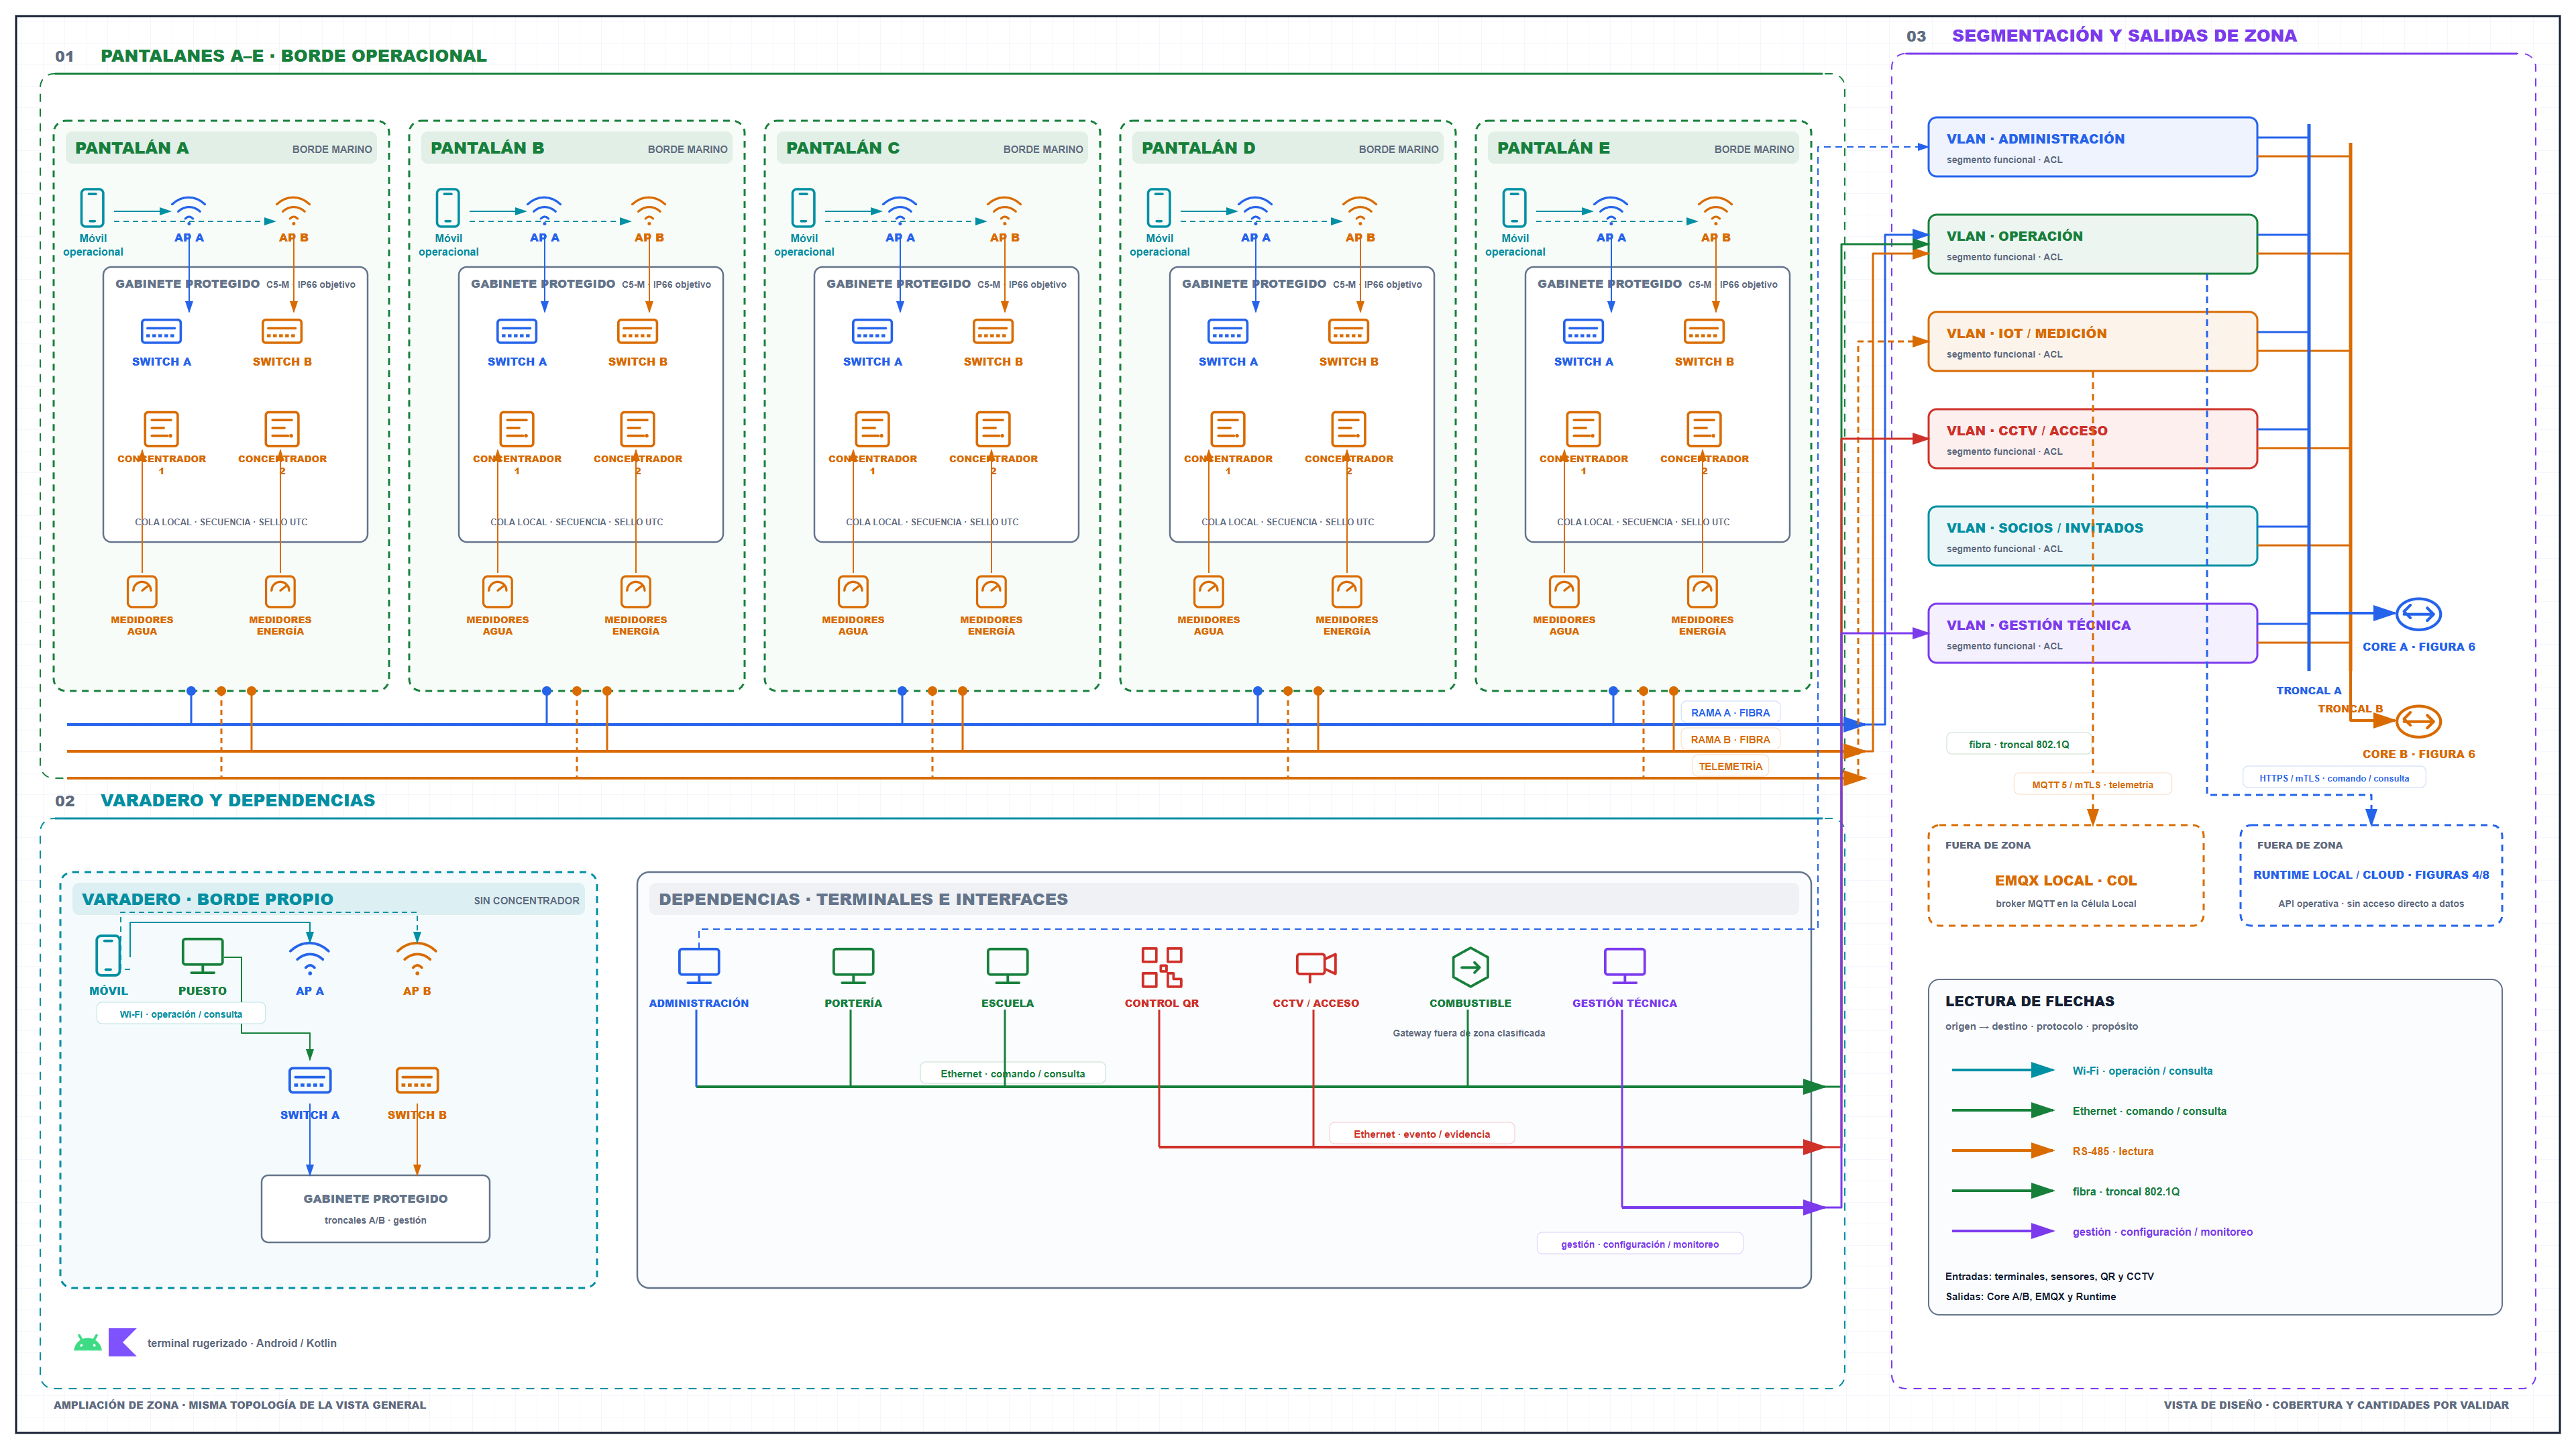
\includegraphics[width=\linewidth,height=.78\textheight,keepaspectratio]{figuras/r8-figura-05.png}
\caption{Terreno, acceso y VLAN.}
\label{fig:r8-5}
\FuenteFigura{Elaboración propia. Vista de diseño sujeta a verificación de sitio, ingeniería y ensayo.}
\end{figure}
\end{paginaHorizontalSynaptix}
\begin{paginaHorizontalSynaptix}
\begin{figure}[H]
\centering
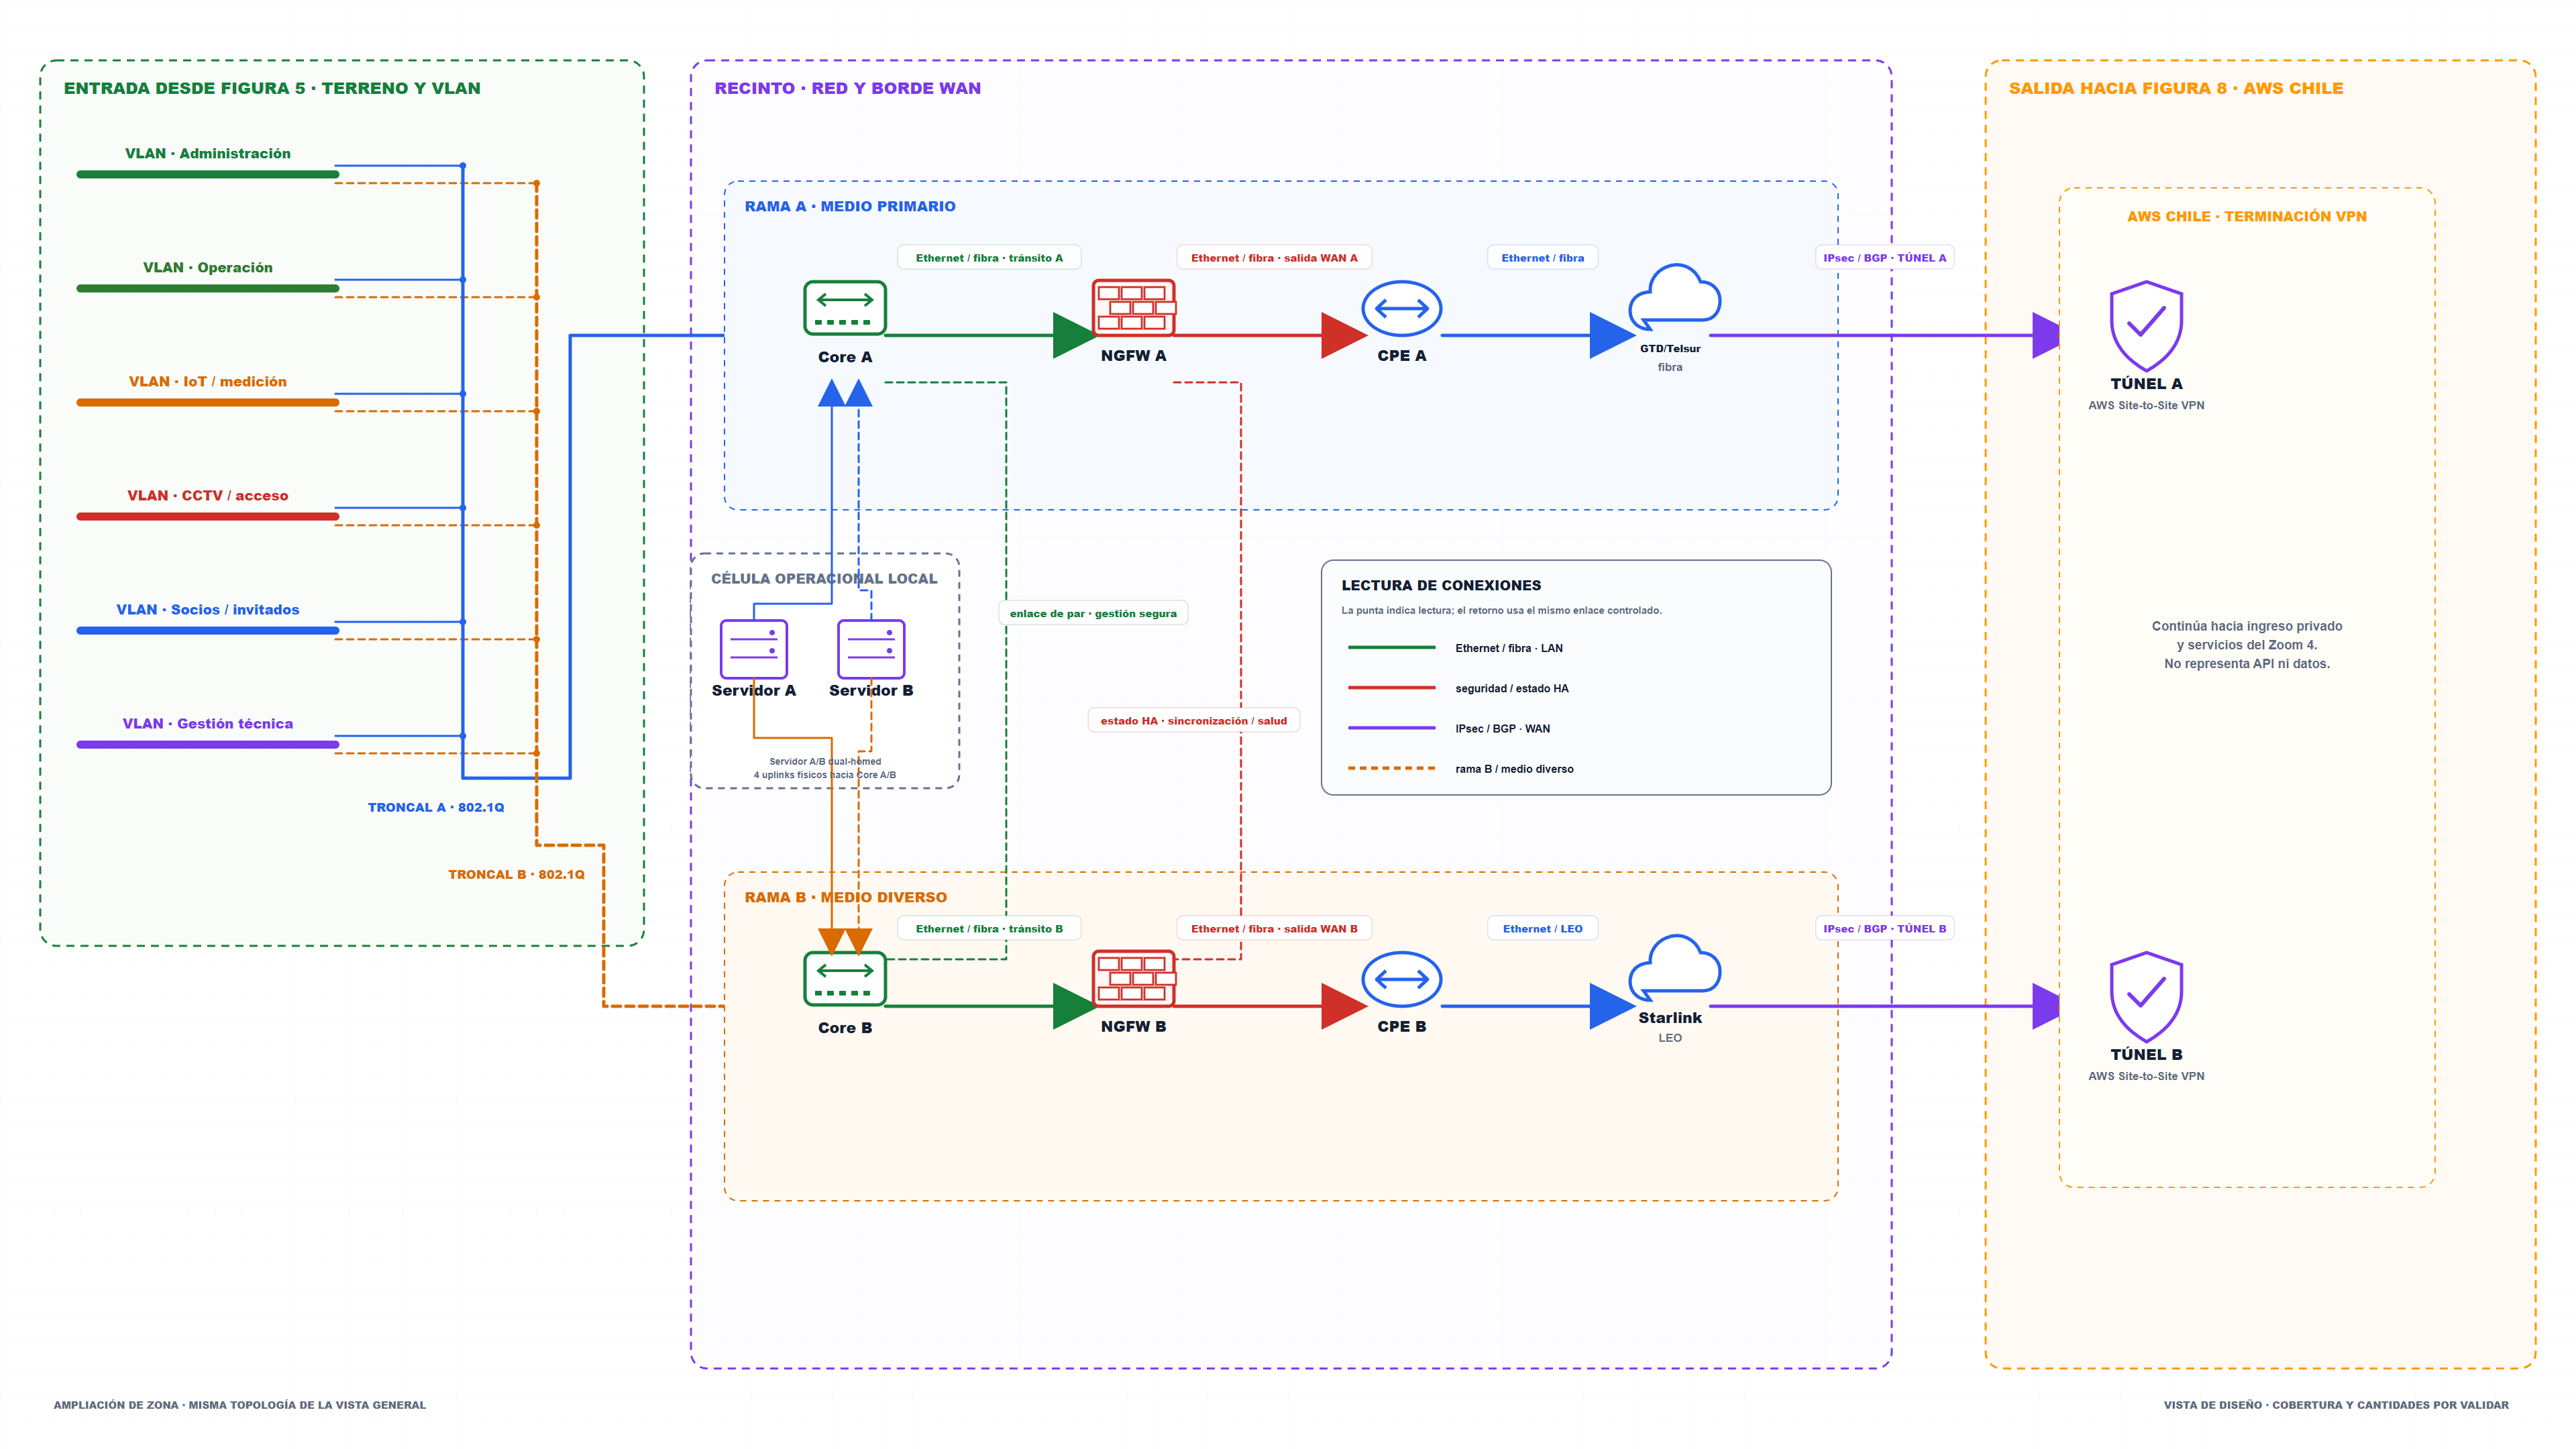
\includegraphics[width=\linewidth,height=.78\textheight,keepaspectratio]{figuras/r8-figura-06.png}
\caption{Red y WAN.}
\label{fig:r8-6}
\FuenteFigura{Elaboración propia. Vista de diseño sujeta a verificación de sitio, ingeniería y ensayo.}
\end{figure}
\end{paginaHorizontalSynaptix}\end{quote}
COL dispone de dos servidores físicos activo/pasivo de 2 U cada uno, cada nodo con al menos cuatro núcleos, 32 GiB, dos SSD empresariales de 1 TB en RAID 1, TPM/gestión remota, doble fuente y dos interfaces; cada nodo sostiene toda la carga crítica. PostgreSQL replica síncronamente entre discos internos de A/B: no depende del almacenamiento auxiliar ni arranca desde él. Se reserva 1 U para el equipo testigo/quorum, con alimentación protegida A/B y control/gestión independiente de los hosts, sujeto a compatibilidad de BOM. Su ubicación en el mismo gabinete no acredita independencia frente a incendio, agua o pérdida total del rack: esos eventos activan contingencia manual y recuperación regional. Pacemaker/Corosync exige quorum y fencing por control independiente de energía/gestión antes de promover. Sin réplica/aislamiento comprobado, no se confirman escrituras automáticas. RAID tolera disco, no reemplaza backup. CIS Ubuntu Level 1 se acredita por reporte/excepciones, y nodos se parchean uno a uno tras prueba.

El almacenamiento auxiliar de 2 U de la figura 4.7 se adopta como destino local de copias restaurables y staging de exportaciones, con al menos 2 TB útiles iniciales, capacidad ampliable y cifra final derivada del corte real/compresión medidos. No aloja el escritor PostgreSQL, WAL, outbox, identidad ni discos de arranque de COL; no es SAN compartida ni requisito de disponibilidad de negocio. Su caída alerta al NOC y suspende esas copias, sin detener transacciones COL; los discos internos conservan hechos y las copias externas siguen su política al estar alcanzables. Acceso por servicio técnico, cifrado, claves recuperables y credenciales separadas; el medio dentro del rack no cuenta como copia fuera de sitio ni acredita por sí solo el segundo medio de 3-2-1-1-0. Modelo, RAID/redundancia y rendimiento quedan sujetos a selección y ensayo.

Falla del activo: detectar/quorum $\rightarrow$aislar $\rightarrow$validar replica $\rightarrow$promover $\rightarrow$probar negocio. Objetivo de conmutación local $\leq$cinco minutos con un solo nodo fallado; límite de restauración local $\leq$dos horas como objetivo más estricto que DR. Si fallan ambos, formularios prenumerados y doble control, sin asignaciones exclusivas remotas; luego digitación/cotejo antes de reabrir. Corte total de energía, disco, LAN, ambos enlaces, reloj, batería, duplica/desorden y conflicto de retiro se ensayan por separado. El procedimiento manual incluye quién decide, qué suspende, custodia, carga y conciliación, no una frase «usar formularios».

\subsection{Especificaciones Implementos a proveer (Hardware y Software)}
El cliente adquiere hardware y ejecuta obras; Synaptix especifica/dimensiona, coordina, configura, integra, administra y mantiene. Integradores especializados instalan/certifican electricidad, zona clasificada y red bajo coordinación Synaptix; fabricante/servicio de terreno reponen equipos. Ninguna tarea técnica normal se asigna a una inexistente área TI de la marina. T-11 local tiene los seis campos oficiales: N°, Categoría/Tipo, Producto/servicio, Ubicación/Lugar, Cantidad y Justificación técnica; los modelos pendientes se distinguen de una especificación comprable (PUCV, 2026a, T-11, p. 62).

El inventario del anexo incluye servicios por ambiente y proveedor aprobado, dos servidores y testigo, firewall/core redundantes, AP/gabinetes, medidores, terminales/puestos, energía y repuestos. La configuración cloud usa referencias de clase verificables antes del gate; el rango de un servicio no sustituye cantidad. La flota móvil comprende seis terminales operacionales para pantalán, tres para escuela, tres para varadero y dos para boyas, total 14, más dos reservas compatibles, total 16. Se adopta como referencia común Samsung Galaxy XCover7 Pro o equivalente acreditado. No se instala en niños ni en botes de escuela. Cada terminal incluye correa, carcasa y base compatibles; cada equipo operacional dispone de batería adicional cuando la variante lo permita, y la carga se organiza de forma segura por turno. La aceptación acredita soporte, SKU local y autonomías de 12 h para terreno y 8 h para boyas; la clasificación IP68 de catálogo no acredita por sí sola aptitud frente a salinidad.

Puestos fijos: 16 operativos +dos reservas, con dos monitores por puesto aplicado y uno de reserva de cada tipo, TPM/cifrado/EDR, gestión central, extraíbles controlados y ergonomía NCh 2527. Distribución: siete administración, dos gerencia/comercial, dos torre, dos portería, uno escuela, uno varadero y uno combustible en oficina segura. Se concilia con turnos/puestos existentes sin afirmar que sean inventario instalado. Los puestos críticos necesitan continuidad eléctrica y tolerancia proporcional a falla; doble fuente/almacenamiento cuando aplica debe verificarse con modelo y no atribuirse a un miniPC de fuente única.

Equipo nuevo y garantía desde recepción, números de serie/firmware/licencias y prueba de puesta en servicio. Hardware crítico: atención en sitio y resolución $\leq$4 h, reemplazo $\leq$4 h desde diagnóstico; no crítico resolución $\leq$24 h hábiles. Repuestos críticos $\geq$10 \% por tipo compatible disponibles en Chile; terreno 10 \% en sitio. Dos nodos, dos firewall y dos core requieren al menos una reserva por tipo si ese es el mínimo entero; HA activa no se cuenta como stock. Medidores iniciales 640 canales ---320 de cada servicio--- implican 32 reservas de agua y 32 de electricidad. Un gateway por cada cinco pantalanes y varadero, seis +una reserva. Modelo físico por servicio/torreta debe conciliar cantidad de dispositivos multicanal con canales, sin doble conteo.

Reposición a 56 meses: firmware/parches según riesgo, baterías móviles cada 24 meses o capacidad <80 \%, UPS según prueba/capacidad y máximo recomendado por fabricante, SSD por desgaste/alarma, medidores recalibrados anualmente o norma aplicable y sustituidos al fallar exactitud, latiguillos/conectores de flexión inspección trimestral/reposición de diseño anual, envolventes/AP/sensores por corrosión/vida útil. Se inventarían accesorios/consumibles y retiro por gestor autorizado; sanitización verificable o destrucción de medios genera certificado. Las frecuencias son hipótesis de oferta a confirmar con fabricante/ambiente, no vida útil certificada.

La carga eléctrica central de diseño para la figura 4.7 considera dos nodos COL de 150 W cada uno, firewall A/B de 30 W cada uno, core A/B de 60 W cada uno, testigo de 15 W, gateway/gestión de 25 W, terminal WAN LEO de 100 W, dos CPE/terminaciones WAN de 15 W cada uno y almacenamiento auxiliar de 50 W; total 700 W. Con una reserva de 25 \%, la potencia de diseño es 875 W y, con factor de potencia 0,9, equivale a 0,972 kVA. Los consumos son cotas propuestas, no mediciones ni fichas acreditadas; si la BOM los excede, se recalcula antes de la compra. El terminal LEO y los CPE son cargas distintas y se contabilizan sin duplicar adaptadores integrados.

Se requieren dos caminos eléctricos A/B, cada uno capaz de toda la carga crítica de 875 W, con protecciones de circuito QF-A/QF-B, UPS online externa $\geq$2 kVA por camino y curva acreditada $\geq$30 min a 875 W por UPS. Cada UPS alimenta su PDU vertical correspondiente. Cada equipo con doble entrada conecta una fuente a A y otra a B; para equipos de una entrada se selecciona transferencia compatible A/B cuya salida al equipo queda identificada. No se conectan entre sí las salidas de UPS ni se suman autonomías de ramas para declarar la de un camino. Transferencia, carga no lineal, tiempo de conmutación, corriente de arranque y compatibilidad de fuentes se verifican con instalador y fabricante. La falla de un camino se ensaya con el otro soportando la carga completa; la transferencia puede ser punto de falla del equipo servido, a gestionar mediante repuesto/contingencia. No se copia una UPS de 60 kVA/centro de datos sin justificarla.

Para 24 h de corte eléctrico de la carga de diseño de 875 W: 0,875$\times$24=21 kWh útiles; con eficiencia 0,90 y descarga admisible 0,80, batería nominal mínima 29,17 kWh por camino capaz de sostener por sí solo esa autonomía. La opción de diseño representada con batería externa A y B exige dos bancos nominales $\geq$30 kWh cada uno ---$\geq$60 kWh total---, con inversor/UPS compatible y capacidad efectiva acreditada considerando envejecimiento/temperatura. No interpretar dos bancos de 15 kWh como 24 h por camino; si ingeniería propone reparto sin esa tolerancia, debe documentar el alcance degradado y aprobar la modificación. La batería integrada de UPS o su banco externo de 30 min no se suma otra vez a estos bancos sin esquema y cálculo de fabricante. Modelo, corrientes, protecciones, segregación, emplazamiento seguro y ensayo quedan pendientes de ingeniería eléctrica. Las 24 h sin nube siguen siendo el compromiso funcional de COL; la autonomía eléctrica extendida es una especificación de diseño separada. Generador sólo mediante cambio calculado y aprobado, no incluido automáticamente.

Gabinetes/AP/gateways de terreno tienen cargas independientes: 12 AP$\times$20 W +seis gateways$\times$15 W =330 W antes de medidores; 25 \% de reserva $\rightarrow$412,5 W, y 24 h a 0,9/0,8 $\rightarrow$13,75 kWh nominales adicionales si deben sostener conectividad completa. Se excluyen del banco central para evitar omisión o doble conteo. La carga se distribuye por gabinete y el consumo real de los instrumentos se mide durante la recepción; la captura móvil con batería permite degradación funcional mientras se recupera Wi-Fi. La autonomía de 24 h sin Internet no se confunde con 24 h sin electricidad, aunque ambos escenarios se ensayan.

Disipación central conservadora 875 W$\times$3,412 $\approx$2.986 BTU/h, antes de pérdidas del respaldo; se considera por zona la ubicación de UPS/bancos externos y cargas fuera del rack. Rango de diseño 18--27 °C/humedad 40--60 \% sujeto a ficha de equipos; sensores de agua/temperatura/humedad e incendio avisan al NOC. Ventilación natural/forzada se evalúa con temperatura de sitio y balance; climatización dedicada sólo se añade si no cumple. UPS/bancos externos quedan segregados, con acceso y protección contra agua/incendio. Puesta a tierra equipotencial/PE, diferenciales, protección galvánica marina y revisión eléctrica semestral se certifican por instalador competente. Mantenimiento preventivo del conjunto trimestral, registro de acceso, pruebas de UPS/bancos y seguimiento de alarmas; inspección eléctrica especializada semestral adicional. Franja libre de servicio de referencia $\geq$1,20 m, a verificar con plano y requisitos aplicables, no como certificación normativa del dibujo.

Gabinete R-01 de referencia 24 U según figura 4.7: patch panel 1 U, organizador 1 U, core A/B 2 U, NGFW A/B 2 U, CPE A/B 2 U, COL A/B 4 U ---2 U cada nodo---, testigo 1 U, almacenamiento auxiliar de copias 2 U y gestión local 1 U; total 16 U ocupadas y ocho U de reserva con tapas ciegas. Distribución: U24 patch, U23 organizador, U22/U21 core, U20/U19 NGFW, U18/U17 CPE, U16--U9 reserva, U8--U7 COL A, U6--U5 COL B, U4 testigo, U3--U2 almacenamiento y U1 gestión. UPS A/B y bancos se emplazan fuera del rack; PDU A/B verticales de 0 U no descuentan la reserva. Las U son envolventes de diseño: profundidad/peso, anclaje, flujo térmico, conectores y tamaños reales deben verificarse con BOM y sitio. El ODF y panelado óptico deben caber en el conjunto de terminación seleccionado o exigir recálculo explícito, sin ocultar unidades adicionales. No se transforma la oficina automáticamente en sala técnica. Obras del cliente incluyen canalizaciones, circuitos, bases/torretas/soporte y certificación; longitudes/condiciones pendientes impiden compra sin especificación completa.

FinOps etiqueta ambiente/módulo/centro de costo, controla presupuesto técnico/alertas y reporte mensual sin imprimir montos. Los ambientes no productivos se apagan programadamente; el escalado evita ociosidad permanente. Huella borde central de diseño: 0,70 kW$\times$8.760 =6.132 kWh/año antes de pérdidas/climatización; terreno AP/gateway $\approx$2.891 kWh/año. PUE se calcula sólo sobre límites de instalación medidos; carbono =energía$\times$factor oficial de red/región registrado por año/proveedor. No se atribuye una reducción de CO2 ni una certificación ISO 14001 sin evidencia.

La figura 4.7 muestra el gabinete R-01: 24 U, 16 U ocupadas y ocho de reserva; PDU verticales de 0 U, UPS y bancos externos. Las cotas son 700/875 W, UPS por rama $\geq$2 kVA y $\geq$30 minutos a carga completa, y bancos A/B $\geq$30 kWh nominales por rama. Compatibilidad, transferencia a entradas únicas y autonomía requieren ingeniería y ensayo. Las 24 horas sin WAN son una condición funcional distinta de la autonomía eléctrica.

\begin{quote}\small \begin{paginaHorizontalSynaptix}
\begin{figure}[H]
\centering
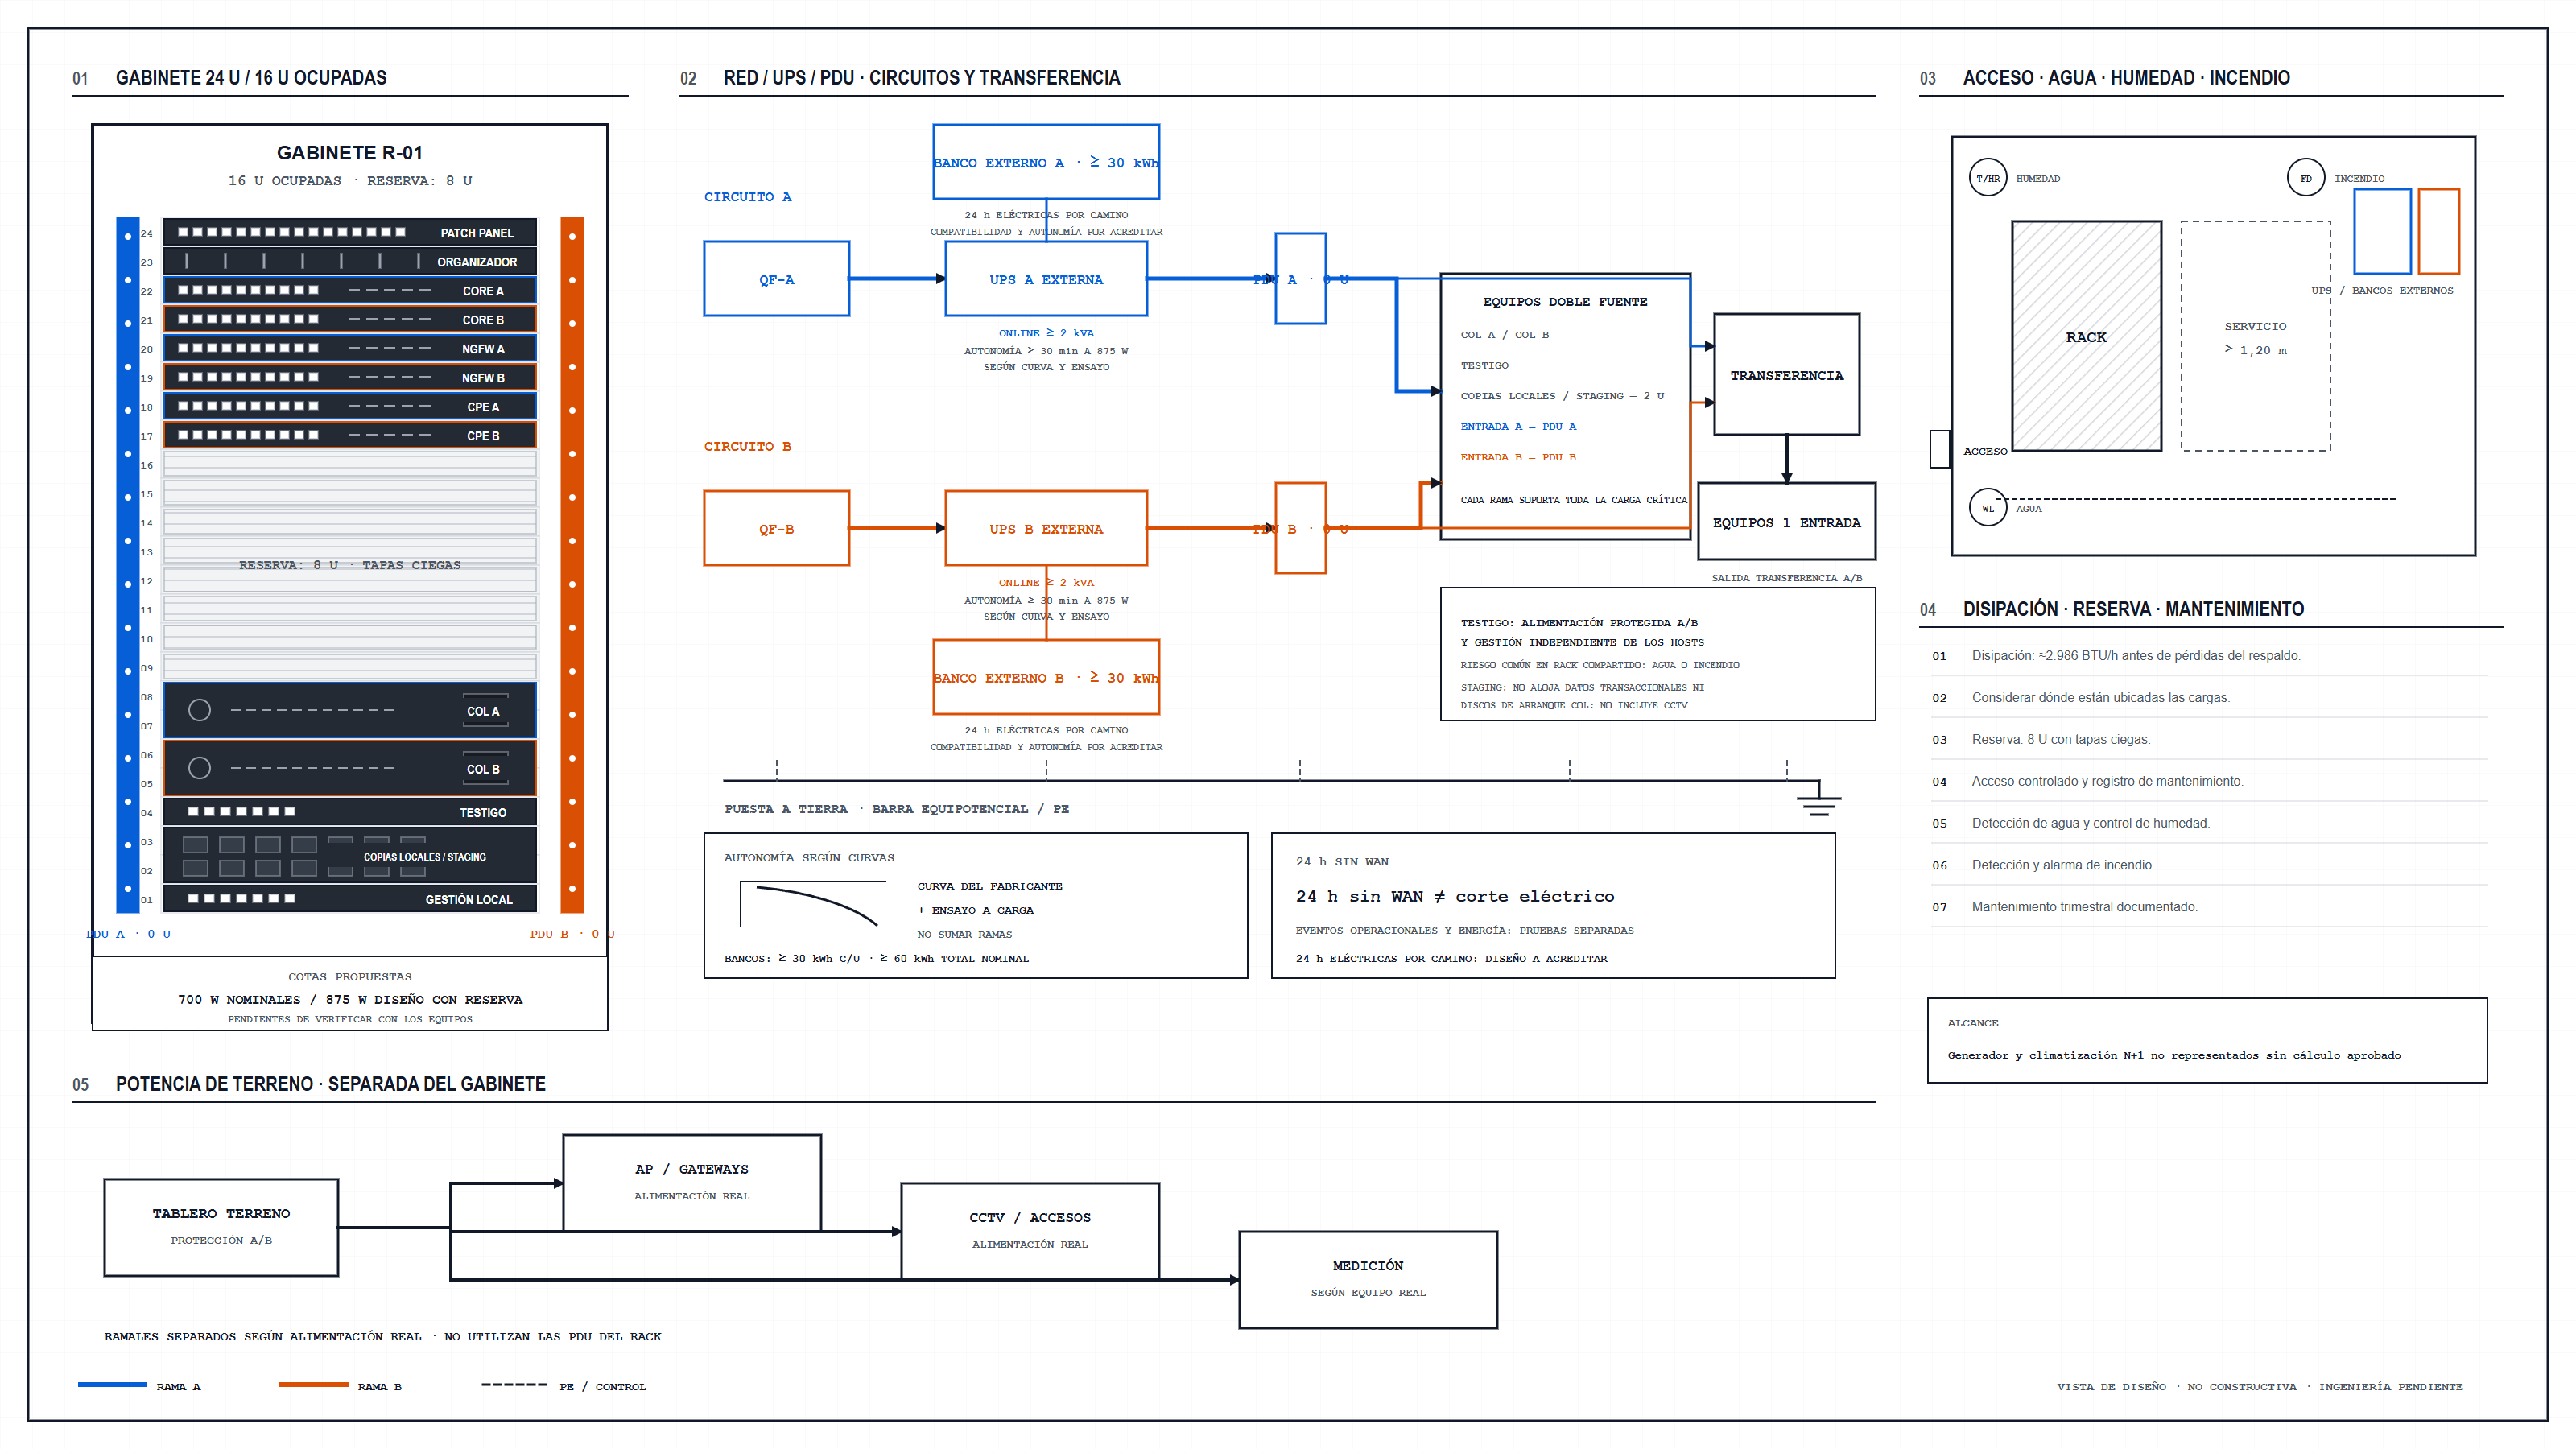
\includegraphics[width=\linewidth,height=.78\textheight,keepaspectratio]{figuras/r8-figura-07.png}
\caption{Gabinete, energía y protecciones.}
\label{fig:r8-7}
\FuenteFigura{Elaboración propia. Vista de diseño sujeta a verificación de sitio, ingeniería y ensayo.}
\end{figure}
\end{paginaHorizontalSynaptix}\end{quote}
\section{Data center}
La estrategia distingue región principal Multi-AZ, DR regional warm standby del mismo proveedor y gabinete mínimo local. HA zonal evita falla de zona; DR cubre pérdida regional; COL cubre pérdida de enlace. Réplica no equivale a copia inmutable y ninguno de esos mecanismos reemplaza la evidencia de aceptación (PUCV, 2026b, caps. 6--7).

\subsubsection*{Gate regional y alternativa contractual}
G-REG se ejecuta antes de H3/mes 6 y, como máximo, al finalizar mes 4 para disponer de dos meses de habilitación/prueba. Arquitectura y operación Synaptix preparan evidencia; seguridad revisa tratamiento y continuidad; Comité de Arquitectura recomienda; representante autorizado del cliente aprueba técnica y contractualmente. Ningún plazo se considera satisfecho por una noticia de anuncio regional.

\begin{table}[H]
\centering
\small
\begin{tabularx}{\linewidth}{|p{.28\linewidth}|X|}
\hline
\EncabezadoTabla{Condición de salida} & \EncabezadoTabla{Evidencia exigida} \\ \hline
Región AWS Chile operativa & Anuncio de disponibilidad general, código real habilitado en cuenta y posibilidad de contratación; no Local Zone ni acceso preliminar. \\ \hline
Dos AZ físicas y capacidad & Identificadores de zona, cuotas y pruebas de creación/despliegue/caída en ambas. \\ \hline
Servicios de la oferta & Disponibilidad real de ECS/Fargate, RDS PG18/Multi-AZ/réplica a São Paulo, S3, SQS, gateway/VPC Link, ALB, KMS/secretos y observabilidad; ingress/CDN con residencia revisada. \\ \hline
Recuperación ejecutable & Warm standby listo, datos/objetos/identidad/claves/mensajes recuperables; prueba real RPO $\leq$15 min/RTO $\leq$4 h. \\ \hline
Contratación y protección & Cuenta/licencias del cliente, soporte, socio acreditado, certificaciones aplicables, subencargados/ubicaciones y autorización escrita. \\ \hline
Hitos y costo & Plan y recursos compatibles con H3; precios sólo en oferta económica; impacto/alternativa firmado por representantes autorizados. \\ \hline
\end{tabularx}
\caption{Gate de habilitación regional}
\label{tab:gate-regional}
\FuenteTabla{criterios de diseño G-REG conforme a PUCV (2026a, arts. 5, 16, 34 y 57; 2026b, RT-03.01/02 y cap. 7)}
\end{table}
La documentación AWS consultada sigue describiendo Chile como lanzamiento previsto para 2026; se conserva expresamente la condición, sin certificar operación actual (AWS, 2025).

Si una condición falla, se documenta brecha e impacto. Se prepara la alternativa GCP Santiago/São Paulo, que debe pasar las mismas pruebas/capacidad/residencia. Activación requiere aprobación contractual; no se inicia por timeout ni automáticamente. Si no existe aprobación o ninguna opción alcanza los objetivos, se eleva desviación al cliente y se revisa el plan; no se rebajan SLA ni se oculta la imposibilidad. No se compran ambos entornos productivos para simular recuperación cruzada.

Santiago/São Paulo se separan aproximadamente 2.600 km en línea recta como referencia geográfica de ciudades, no coordenadas de edificios ni certificación de distancia física exacta. Gate conserva ubicación/certificación real que el proveedor permita acreditar. Amenazas comunes: identidad/configuración, borrado lógico, credenciales, operador/comunicaciones internacionales y control global del proveedor. Sismo/inundación/energía se analizan por sitios/regiones; no se declara ausencia de correlación. Copias independientes, claves/cuentas separadas y COL limitan esos riesgos. T-7 solicita especificación/certificación aplicable Tier/ANSI-TIA-942; reportes genéricos ISO del proveedor no acreditan por sí solos un edificio. Socio certificado/acuerdo formal y evidencias específicas continúan como antecedentes externos.

\subsection{Especificaciones Data Center Primaria}
AWS Chile/Santiago es el primario objetivo, sujeto a G-REG, con dos AZ físicas como mínimo para componentes HA. Tras aprobación se registra código, zonas, servicios/clases/quotas y capacidad contractual. Tres aplicaciones y sus trabajadores se distribuyen entre zonas; el balanceador y RDS transaccional tienen redundancia. Amazon Cognito administra identidad como servicio regional y su continuidad se verifica separadamente mediante el pool de contingencia. El standby zonal de RDS no se cuenta como escritor adicional. Objetos cifrados/versionados, políticas de red/cuentas, claves/secretos, auditoría y respaldo están protegidos por responsabilidad compartida: proveedor protege instalaciones/plataforma; Synaptix protege configuración/aplicación/identidades/datos y recuperación.

Si se aprueba GCP, Santiago southamerica-west1 ocupa ese papel, con Cloud Run regional, Cloud SQL HA, identidad en dos zonas, storage regional y gateway/control equivalentes. La COL continúa igual en ambas alternativas. Se verifican tratamientos externos y plano de control; «regional» no permite afirmar que todo metadato o servicio global reside exclusivamente en esa región.

El recinto se clasifica como gabinete/borde operacional gestionado; sólo incorpora cómputo/red/energía necesarios. Cierre físico, ingreso autorizado/bitácora y acompañamiento de terceros, detección de agua/temperatura/humo y medios de extinción apropiados al riesgo se definen con instalador/seguridad. Requisitos de sala técnica no aplicables a gabinete se justifican individualmente; no se omite protección por cambiar la etiqueta. Respaldos automáticos evitan traslado semanal manual de discos por la marina. Disponibilidad de infraestructura 99,95 \% y crítico de extremo a extremo 99,9 \% se miden por separado; cumplir uno no demuestra el otro.

La figura 4.8 detalla AWS Chile como región principal condicionada a G-REG: ingreso protegido, Amazon Cognito, API Gateway REST/VPC Link V2/ALB privado, aplicaciones distribuidas en dos AZ y RDS Multi-AZ. Ambas AZ acceden al endpoint writer; el standby recibe réplica y no escrituras de las aplicaciones. Route 53 resuelve DNS y no constituye un salto de tráfico HTTPS.

\begin{quote}\small \begin{paginaHorizontalSynaptix}
\begin{figure}[H]
\centering
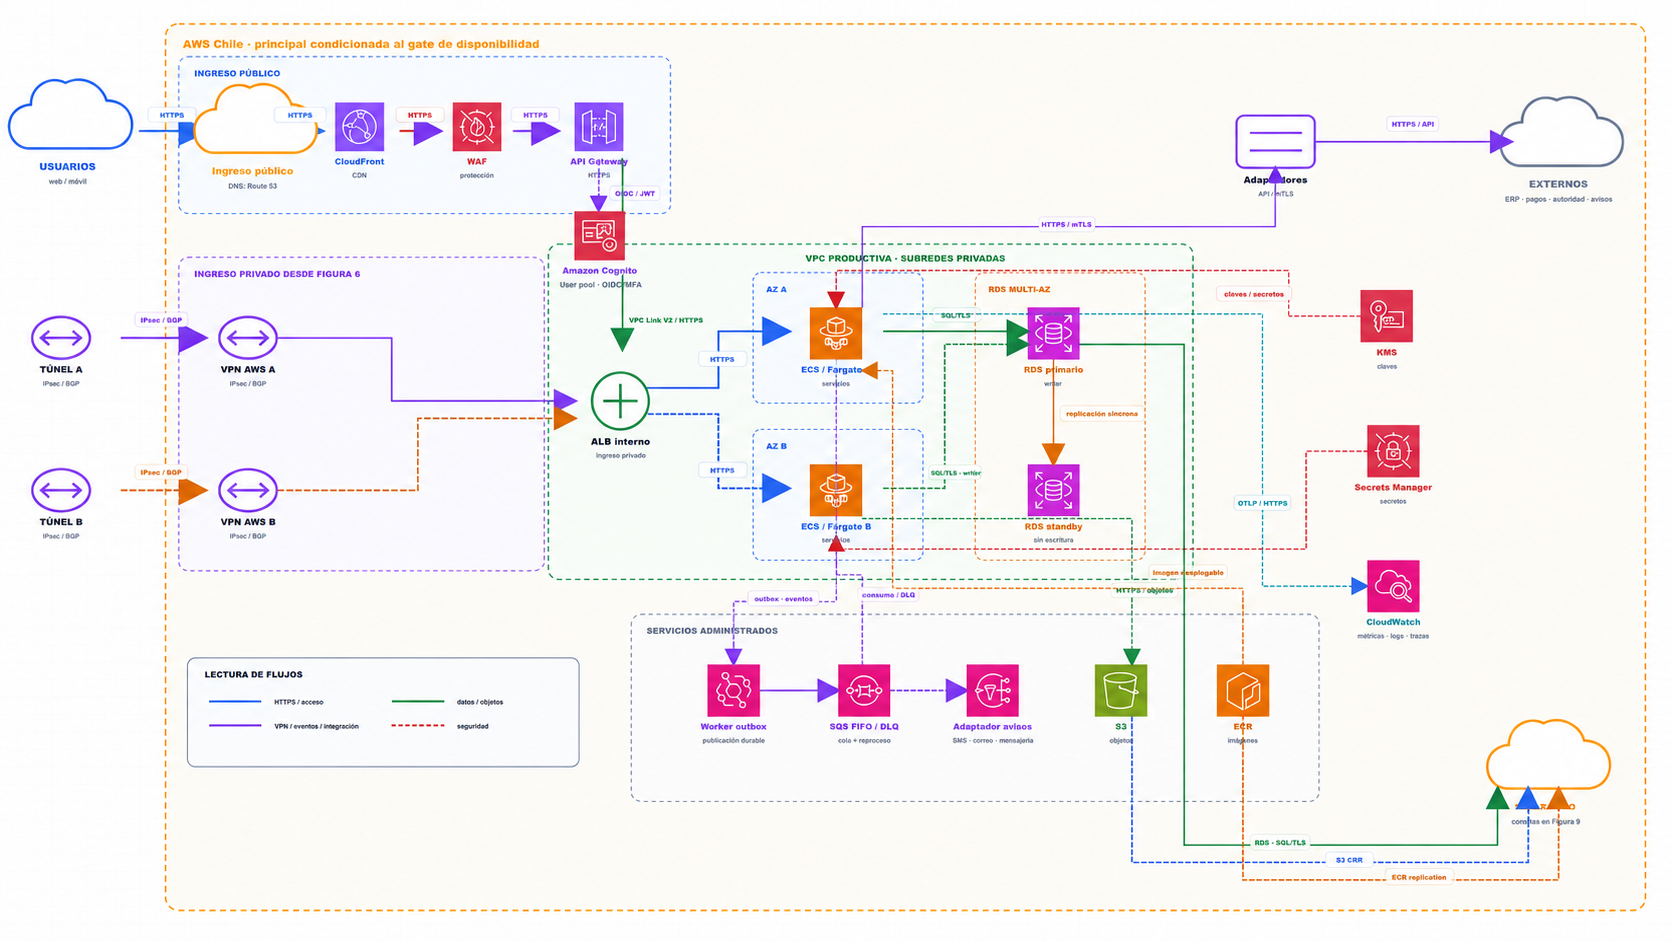
\includegraphics[width=\linewidth,height=.78\textheight,keepaspectratio]{figuras/r8-figura-08.png}
\caption{AWS Chile: región principal condicionada.}
\label{fig:r8-8}
\FuenteFigura{Elaboración propia. Vista de diseño sujeta a verificación de sitio, ingeniería y ensayo.}
\end{figure}
\end{paginaHorizontalSynaptix}\end{quote}

\subsection{Especificaciones Data Center Secundario}
AWS São Paulo sa-east-1 mantiene warm standby si AWS Chile supera G-REG. Si se activa GCP, su secundario es São Paulo southamerica-east1, también warm standby. El secundario tiene red, ingress, certificados, contenedores, identidad, claves, almacenamiento y capacidad mínima habilitados antes de producción; los datos se replican continuamente y escala a capacidad productiva al promover. No se mantiene un secundario operacional en el proveedor alternativo.

AWS replica RDS PostgreSQL entre regiones mediante réplica de lectura promovible con funcionalidad/regiones verificadas; objetos se replican con manifiestos/huellas y atraso medido. La configuración autorizada de Cognito se versiona y aplica al user pool de contingencia; las identidades federadas vuelven a autenticarse y las cuentas no federadas requieren enrolamiento de recuperación previo, sin afirmar réplica de contraseñas. SQS no se copia como estado mágico: el corte de outbox/inbox y la deduplicación reconstruyen pendientes en colas del secundario. GCP usa réplica interregional Cloud SQL promovible, objetos regionales y despachador sobre outbox/inbox; no supone intercambio SQS/PubSub. HA y promoción DR son mecanismos diferentes (AWS, s. f.-c; Google Cloud, s. f.-b).

RPO $\leq$15 min se mide desde último hecho durable cloud hasta corte recuperado, con heartbeat por minuto y retraso de objetos/identidad además de LSN. Aviso a cinco minutos, incidente preventivo a diez y escalamiento crítico al alcanzar 15. Hechos nuevos de COL desconectada siguen locales y no forman parte de un RPO cloud falsamente actualizado; se reconcilian al volver. Los cinco minutos de supervisión no autorizan ignorar una réplica atrasada.

RTO $\leq$4 h comienza con declaración de interrupción del servicio crítico y termina con validación de transacciones/usuarios del alcance crítico en DR. Presupuesto de diseño: detección/decisión 30 min, aislamiento/promoción 30, activación/adaptadores/identidad 45, validación 45 y apertura 30; total 180 min, 60 de reserva. Escalar desde cero, descargar copias o enrolar todos los usuarios durante incidente no es warm standby aceptable.

Failover: NOC registra incidente $\rightarrow$ responsable de continuidad/cliente autoriza $\rightarrow$ se bloquea o acredita aislamiento de escritura primaria $\rightarrow$ verifica corte/objetos/identidad $\rightarrow$promueve datos $\rightarrow$actualiza endpoints/secretos y activa consumidores $\rightarrow$prueba salida/retiro/amarra/despacho/cuenta $\rightarrow$abre tráfico y comunica restricciones. Sin aislamiento/corte conocido se mantiene contingencia segura y no doble escritor. DNS tiene TTL de diseño 60 s; se mide propagación real. Failback es planificado: resembrar primario desde sitio vigente, validar conteos/huellas, drenar pendientes, ventana aprobada y retorno reversible. No se reutiliza una réplica divergente.

Antes de producción y al menos dos veces/año se realiza conmutación real con informe RTO/RPO y cierre de brechas; restauración de muestra representativa mensual con tiempo registrado. Ningún ensayo previsto se presenta ejecutado. Escenarios incluyen zona/región, identidad, objetos, cola, réplica retrasada, ambos enlaces, COL/disco/energía y error humano/borrado. Crítico/alto/medio/bajo: disponibilidades 99,9/99,5/99,0/98,0 \%, respuesta 15 min/1 h/4 h/8 h y resolución 4/8/24/48 h, con cobertura acordada. ISO 22301/27031 guían BIA/runbooks, sin afirmar certificación.

Respaldo 3-2-1-1-0: dato productivo, copia restaurable independiente y copia externa; se exige acreditar dos medios/plataformas de almacenamiento realmente independientes, al menos una inmutable/offline y cero errores de verificación. La diversidad entre tabla y archivo no demuestra dos medios físicos. Objetos con Object Lock/retención equivalente, cuenta de backup separada, claves independientes y privilegios sin borrado limitan compromiso administrativo. El medio adicional independiente y servicio/ubicación se deben contratar/acreditar; hasta entonces 3-2-1-1-0 queda pendiente de evidencia, no conforme por enunciado.

Política inicial: transaccional/identidad PITR 35 días, copia diaria 35, mensual 12 y anual según mayor retención de dominio; COL diario 30 días y copia crítica al volver enlace; configuración/IaC cada cambio y diario; objetos conforme a clase y legal hold; logs/auditoría por sus plazos. Volumen de copia se deriva del corte real y factor de compresión medido; se dimensiona hasta tres copias sin sumar réplica como inmutable. Restauración completa se prueba con datos, permisos, claves, dispositivos e identidad, y reaplica eliminaciones legítimas antes de abrir.

La figura 4.9 muestra recuperación en AWS São Paulo mediante warm standby y promoción autorizada, sin doble escritura. Incluye el user pool de Cognito de contingencia, objetos, claves y reconstrucción de mensajes desde outbox/inbox con sincronización COL. RPO $\leq$15 minutos y RTO $\leq$4 horas son objetivos por ensayar. Las copias inmutables siguen la política descrita y no se confunden con réplica regional; la lámina sintetiza failover/failback y no detalla todos los medios de respaldo.

\begin{quote}\small \begin{paginaHorizontalSynaptix}
\begin{figure}[H]
\centering
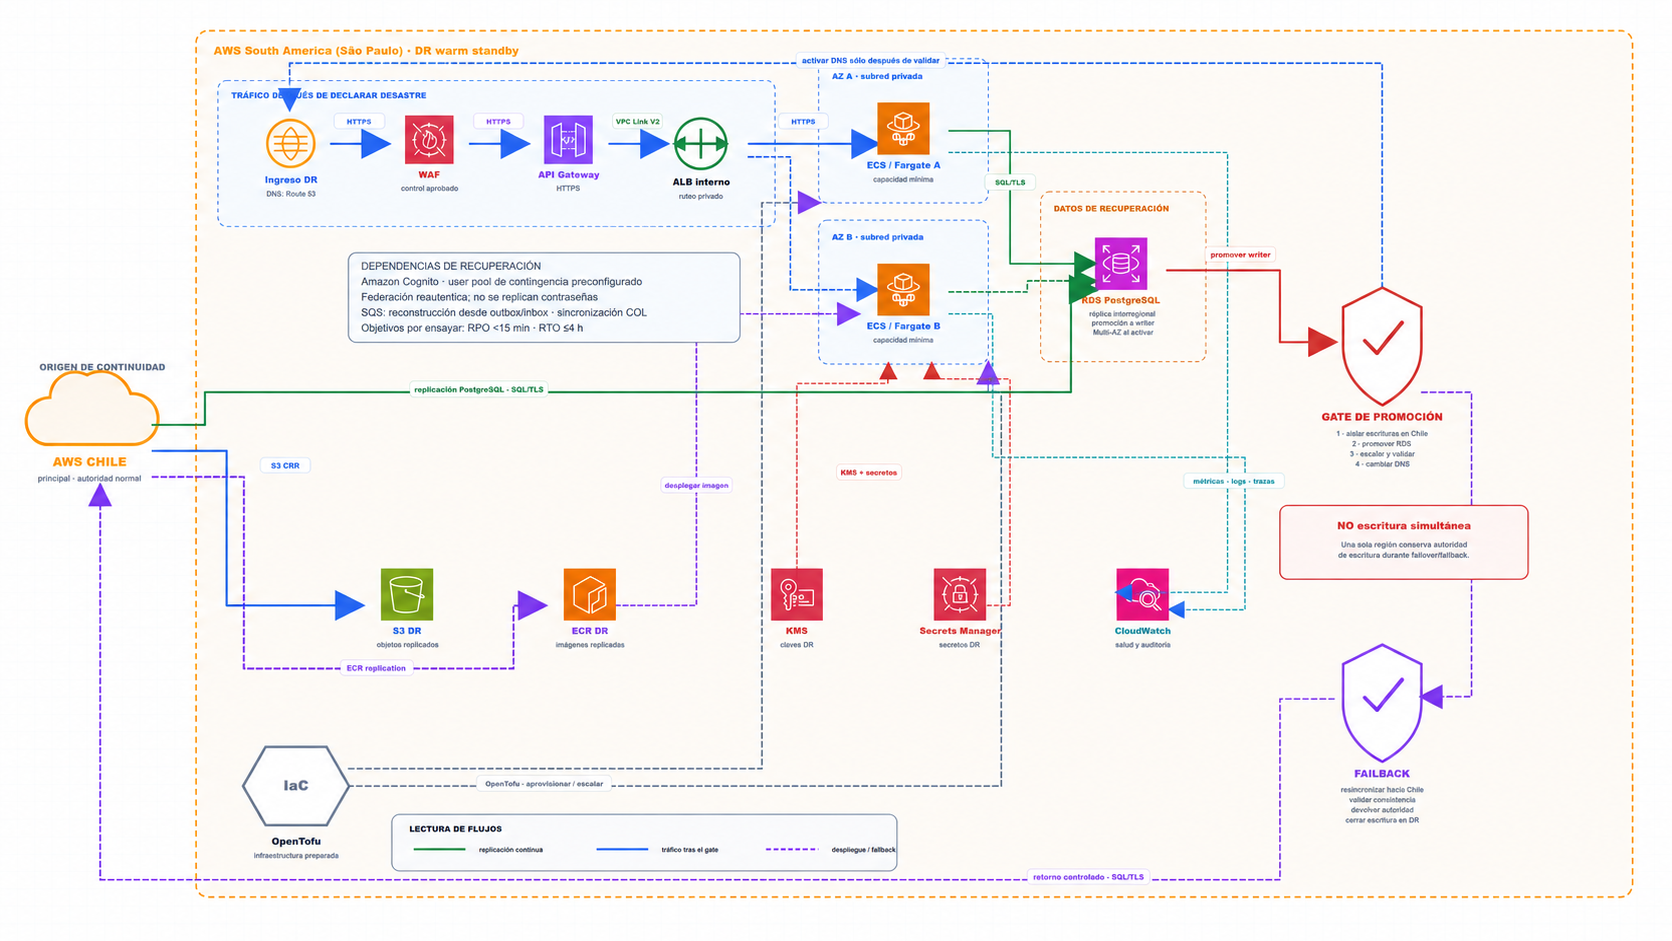
\includegraphics[width=\linewidth,height=.78\textheight,keepaspectratio]{figuras/r8-figura-09.png}
\caption{AWS São Paulo: recuperación warm standby.}
\label{fig:r8-9}
\FuenteFigura{Elaboración propia. Vista de diseño sujeta a verificación de sitio, ingeniería y ensayo.}
\end{figure}
\end{paginaHorizontalSynaptix}\end{quote}
\subsubsection*{Gobierno, decisiones, reversibilidad e innovaciones}
El Comité de Arquitectura aplica un gobierno equivalente a TOGAF adaptado: requisitos/preocupaciones $\rightarrow$vistas $\rightarrow$alternativas/ADR $\rightarrow$revisión técnica/seguridad/datos $\rightarrow$cambio aprobado $\rightarrow$pruebas/hitos y seguimiento. Cada ADR fechado conserva elección, alternativas, criterio, fundamento, impacto y validación; no basta sustituir LB-V por «cerrado». El anexo relaciona las 22 decisiones del caso con su consecuencia arquitectónica y evidencia pendiente. T-12 global debe cubrir 374 RT según su documento/numeral/texto, distinguiendo códigos homónimos CAS/BT; sólo lo arquitectónico se desarrolla aquí.

Administrador funcional propuesto: cargo de jefatura administrativa, con suplencia de jefatura de operaciones designada por cliente; nombres no se inventan. Estimación mensual: usuarios/altas cuatro horas, catálogos/reglas cuatro, conciliación/excepciones ocho, contactos/consentimientos cuatro, coordinación/aceptaciones cuatro y revisión de reportes cuatro =28 horas-persona/mes. En temporada se reserva 25 \% adicional, 35 HP/mes. Son hipótesis con frecuencia y sustitución; Synaptix realiza parches/backups/proveedores/monitoreo, no esos cargos. La designación y disponibilidad reales deben confirmarse.

IN1 solicitudes de mantenimiento e IN2 mantenimiento programado durante invernada usan IN1-SOL, AUT/CTR/VAR/ALE y clientes/contratos; no crean órdenes duplicadas. IN3 extracción documental asistida utiliza repositorio $\rightarrow$adaptador aislado $\rightarrow$propuesta de campos $\rightarrow$aprobación humana ADM $\rightarrow$datos aprobados NAV, con privacidad y fallback manual. IN4 es el Servicio Gestionado por Resultados: IN4-MET mide tiempo activo, errores y cierre del seguimiento de solicitudes; IN4-CON conserva expediente/acta de conciliación para que el cliente acepte un incentivo adicional, sin modificar el SLA base ni autorizar un pago sólo por tablero. IN5 es el plan voluntario de reducción de agua por embarcación: IN5-HIS proyecta la serie común validada, IN5-PLAN conserva acción/responsable/plazo/evidencia y compara períodos equivalentes; no corta suministro ni certifica una nave. Todas usan ambientes, eventos/seguridad, volumen y pruebas del núcleo. Los códigos internos IN1--IN5 y sus paquetes deben corresponder al SD13/SD7 definitivo; las fechas exactas de cada innovación se concilian, no se inventan. No se presenta el estado multifuente obligatorio como innovación adicional.

Reversibilidad: inventario distingue portables ---código, contenedores, PostgreSQL, contratos, Parquet/objetos/metadatos y Terraform--- de adaptadores propietarios ---gateway, mensajería, IAM/KMS/monitorización---. Exportación completa y ejecución por tercero incluyen identidad/credenciales autorizadas, licencias y runbooks, no sólo base. Hipótesis de migración controlada: 40 HP inventario, 80 adaptación, 40 transferencia/conciliación y 40 pruebas =200 HP, a validar con volumen/integraciones; sin precios aquí. Plan inicial dentro de primeros 90 días, actualización anual y acompañamiento mínimo 90 días al terminar. Cambio de GCP a AWS exige además aprobación/ensayo de migración, no se confunde con DR.

\section*{Referencias}
\addcontentsline{toc}{section}{Referencias}
Las bases se citan por documento/año/numeral; el plan suministrado orienta la revisión y no sustituye las fuentes. Las referencias técnicas siguientes sustentan sólo las capacidades que se utilizan; no acreditan adquisición, aprobación ni ensayo. Consultas web: 10 de octubre de 2026.

\noindent\textbullet\ Pontificia Universidad Católica de Valparaíso. (2026a). Bases Administrativas TFEP-01/2026 (FEP01.26). Arts. 5, 16--29, 34, 46, 50, 57, 71--85; T-7/T-11/T-12/T-22.\par
\noindent\textbullet\ Pontificia Universidad Católica de Valparaíso. (2026b). Bases Técnicas Transversales TFEP-01/2026 (FEP02.26). Caps. 2--18 y 20--21. La referencia por RT se acompaña del documento para evitar códigos homónimos.\par
\noindent\textbullet\ Pontificia Universidad Católica de Valparaíso. (2026c). Bases Técnicas del Caso 07: Servicio de Puerto Deportivo. Caps. 9--18; volumetría pp. 30--31; condiciones pp. 33--36; asuntos §17.4 pp. 41--42.\par
\noindent\textbullet\ Pontificia Universidad Católica de Valparaíso. (2026d). Comunicado 10 e instrucciones complementarias de estructura de la propuesta. Apartados 2--7 y capítulo 4.\par
\noindent\textbullet\ Amazon Web Services. (2025, 7 de mayo). In the works -- AWS South America (Chile) Region. \url{https://aws.amazon.com/blogs/aws/coming-soon-aws-south-america-chile-region/}\par
\noindent\textbullet\ Amazon Web Services. (s. f.-a). AWS Chile. \url{https://aws.amazon.com/es/local/chile/}\par
\noindent\textbullet\ Amazon Web Services. (s. f.-b). Private integrations for REST APIs in API Gateway. \url{https://docs.aws.amazon.com/apigateway/latest/developerguide/private-integration.html}\par
\noindent\textbullet\ Amazon Web Services. (s. f.-c). Working with read replicas for Amazon RDS for PostgreSQL. \url{https://docs.aws.amazon.com/AmazonRDS/latest/UserGuide/USER\_PostgreSQL.Replication.ReadReplicas.html}\par
\noindent\textbullet\ Google Cloud. (s. f.-a). Cloud Run locations. \url{https://docs.cloud.google.com/run/docs/locations}\par
\noindent\textbullet\ Google Cloud. (s. f.-b). Promote replicas for regional migration or disaster recovery. \url{https://docs.cloud.google.com/sql/docs/postgres/replication/cross-region-replicas}\par
\noindent\textbullet\ Google Cloud. (s. f.-c). Database versions and version policies. \url{https://docs.cloud.google.com/sql/docs/postgres/db-versions}\par
\noindent\textbullet\ PostgreSQL Global Development Group. (s. f.). Versioning policy. \url{https://www.postgresql.org/support/versioning/}\par
\noindent\textbullet\ Amazon Web Services. (s. f.-d). Amazon Cognito user pools. \url{https://docs.aws.amazon.com/cognito/latest/developerguide/cognito-user-pools.html}\par
\noindent\textbullet\ Spring. (s. f.). System requirements. \url{https://docs.spring.io/spring-boot/system-requirements.html}\par
\noindent\textbullet\ Starlink. (s. f.). Business: Fixed sites. \url{https://starlink.com/business/fixed-site}\par
\noindent\textbullet\ Rose, S., Borchert, O., Mitchell, S., \& Connelly, S. (2020). Zero trust architecture (NIST SP 800-207). \url{https://doi.org/10.6028/NIST.SP.800-207}\par
\section*{Declaración de uso de IA}
\addcontentsline{toc}{section}{Declaración de uso de IA}
OpenAI Codex se utilizó como herramienta de apoyo para estructurar contenidos, contrastar documentación técnica y asistir en la redacción. Las decisiones de arquitectura, cantidades, cálculos, fuentes y condiciones de aceptación deben ser verificadas y aprobadas por el responsable humano antes de la emisión. Este uso es independiente de IN3, funcionalidad de IA propuesta para el sistema.

\begin{table}[H]
\centering
\small
\begin{tabularx}{\linewidth}{|p{.12\linewidth}|p{.21\linewidth}|p{.10\linewidth}|p{.16\linewidth}|X|}
\hline
\EncabezadoTabla{Sección / soporte} & \EncabezadoTabla{Herramienta / finalidad} & \EncabezadoTabla{Texto} & \EncabezadoTabla{Diagramas} & \EncabezadoTabla{Revisión humana} \\ \hline
Capítulo 4/4.1 & Codex; arquitectura, controles y procesos & Alto & Nueve láminas incorporadas & Verificación técnica requerida antes de emisión. \\ \hline
4.1.1 & Codex; selección, soporte y contraste documental & Alto & Ninguno & Verificación documental requerida antes de emisión. \\ \hline
4.2/4.2.1 & Codex; despliegue, fórmulas e inventario & Alto & Nueve láminas incorporadas & Verificación de cantidades, cálculos y condiciones del sitio requerida antes de emisión. \\ \hline
4.3 y subapartados & Codex; condiciones de habilitación y recuperación regional & Alto & Nueve láminas incorporadas & Aprobación técnica y ensayo requeridos conforme al plan de aceptación. \\ \hline
Anexo A4 & Codex; contratos, amenazas, ADR y trazabilidad & Alto & Ninguno & Verificación de coherencia documental requerida antes de emisión. \\ \hline
\end{tabularx}
\caption{Uso de IA y revisión humana}
\label{tab:uso-ia}
\FuenteTabla{registro de elaboración del subdocumento}
\end{table}
El Formulario A-6 debe reflejar el uso efectivo de herramientas y la verificación humana realizada. Antes de la entrega, el responsable designado debe validar arquitectura, supuestos, cálculos, privacidad, fuentes y coherencia. Las pruebas y resultados de ejecución se acreditarán en los hitos correspondientes.


\end{document}
